\documentclass[aspectratio=169]{beamer}
\usetheme{Madrid}
\usecolortheme{default}
\usepackage[utf8]{inputenc}
\usepackage[T5]{fontenc}
\usepackage{graphicx}
\usepackage{hyperref}
\usepackage{booktabs}
\usepackage{amsmath}

% Setup for code listings
\usepackage{listings}
\usepackage{xcolor}
\definecolor{codegreen}{rgb}{0,0.6,0}
\definecolor{codegray}{rgb}{0.5,0.5,0.5}
\definecolor{codepurple}{rgb}{0.58,0,0.82}
\definecolor{backcolour}{rgb}{0.95,0.95,0.92}
\lstdefinestyle{mystyle}{
    backgroundcolor=\color{backcolour},   
    commentstyle=\color{codegreen},
    keywordstyle=\color{magenta},
    numberstyle=\tiny\color{codegray},
    stringstyle=\color{codepurple},
    basicstyle=\ttfamily\scriptsize,
    breakatwhitespace=false,         
    breaklines=true,                 
    captionpos=b,                    
    keepspaces=true,                 
    numbers=left,                    
    numbersep=5pt,                  
    showspaces=false,                
    showstringspaces=false,
    showtabs=false,                  
    tabsize=2
}
\lstset{style=mystyle}

\setbeamertemplate{caption}[numbered]
\renewcommand{\figurename}{Hình}
\renewcommand{\thefigure}{5.\arabic{figure}}

\title[Chương 5: Nền tảng Học máy]{Học Sâu (Deep Learning) \\ \vspace{0.5cm} \Large Chương 5: Nền tảng của Học máy (Fundamentals of ML)}
\author{Đại học Đông Á}
\date{\today}

\begin{document}

\begin{frame}
    \titlepage
\end{frame}

\begin{frame}{Nội dung chương}
    \tableofcontents
\end{frame}

\section{1. Tối ưu hóa (Optimization) và Khái quát hóa (Generalization)}

\begin{frame}{Sự giằng co cốt lõi trong Học máy}
    \begin{itemize}
        \item \textbf{Tối ưu hóa (Optimization):} Quá trình điều chỉnh mô hình để đạt hiệu suất tốt nhất trên tập dữ liệu huấn luyện (\textit{Training data}).
        \item \textbf{Khái quát hóa (Generalization):} Khả năng mô hình dự đoán chính xác trên dữ liệu hoàn toàn mới chưa từng thấy (\textit{Test data}).
        \item \textbf{Mục tiêu:} Đạt được khả năng Generalization cao nhất. Tuy nhiên, thuật toán Gradient Descent chỉ có thể trực tiếp tác động vào quá trình Optimization.
        \item \textbf{Mâu thuẫn:} Sau một thời gian huấn luyện nhất định, Optimization càng tốt thì Generalization lại càng đi xuống.
    \end{itemize}
\end{frame}

\begin{frame}{Hiện tượng Underfitting và Overfitting}
    \begin{columns}
        \column{0.5\textwidth}
        \begin{itemize}
            \item \textbf{Underfitting (Chưa khớp):} Mô hình quá đơn giản, không học được quy luật trong dữ liệu. (Ví dụ: Dùng đường thẳng tuyến tính để khớp dữ liệu phân bố parabol).
            \item \textbf{Robust Fit (Khớp chuẩn):} Mô hình học được xu hướng thực sự của dữ liệu.
            \item \textbf{Overfitting (Quá khớp):} Mô hình quá phức tạp, học thuộc lòng cả các "nhiễu" (noise) của dữ liệu huấn luyện, khiến đường biên quyết định cong queo, mất đi tính tổng quát.
        \end{itemize}
        
        \column{0.5\textwidth}
        \begin{figure}
            \centering
            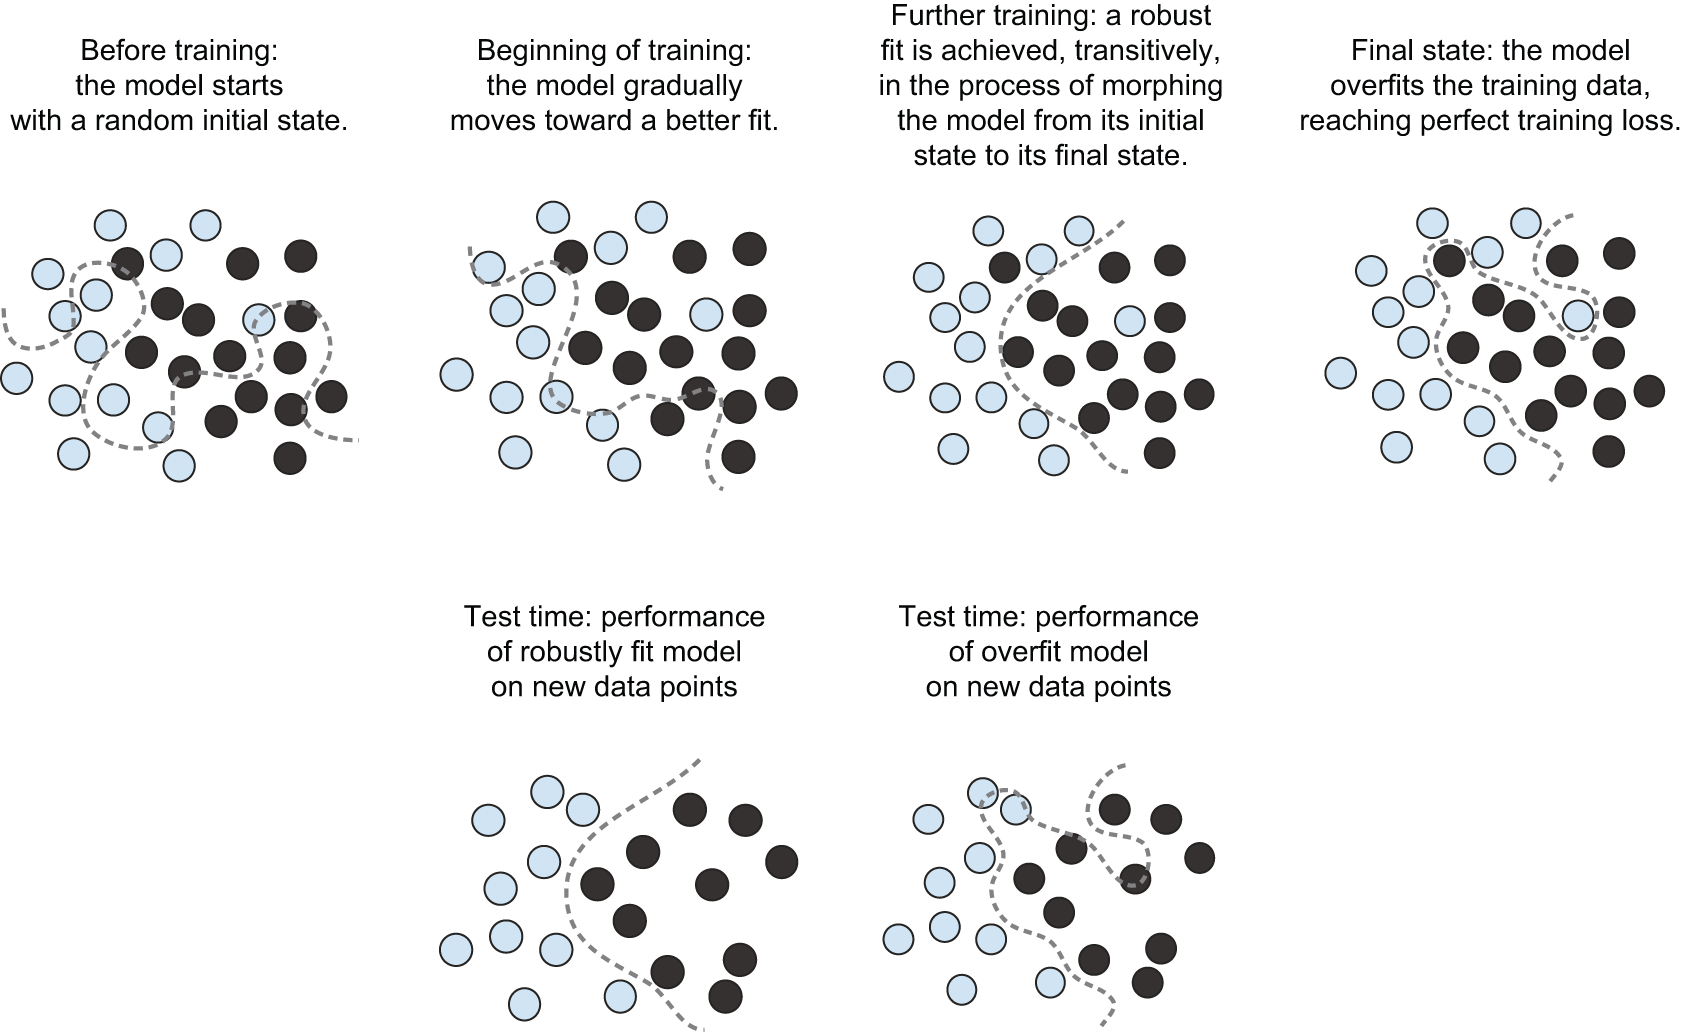
\includegraphics[width=\textwidth,height=0.7\textheight,keepaspectratio]{../../images/ch05/the_cartoon_of_fitting.096e7b07.png}
            \caption{Mô phỏng Underfitting, Robust Fit và Overfitting}
        \end{figure}
    \end{columns}
\end{frame}

\begin{frame}{Vòng đời điển hình của mô hình (Universal Overfitting)}
    \begin{columns}
        \column{0.5\textwidth}
        \begin{itemize}
            \item Ở giai đoạn đầu, Loss trên tập Train và tập Validation cùng giảm, các tham số đang liên tục điều chỉnh đúng hướng $\rightarrow$ Giai đoạn Underfitting.
            \item Sau một số epoch nhất định, Validation Loss bắt đầu chững lại và tăng vọt trở lại, dù Training Loss vẫn tiếp tục giảm tiệm cận 0 $\rightarrow$ \textbf{Giai đoạn Overfitting}.
        \end{itemize}
        
        \column{0.5\textwidth}
        \begin{figure}
            \centering
            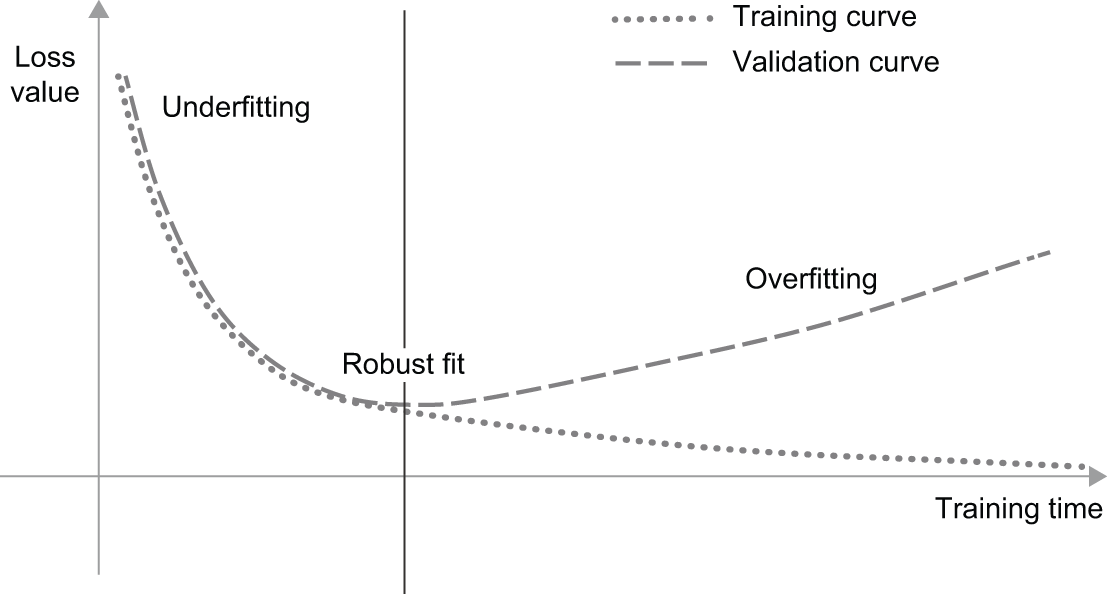
\includegraphics[width=\textwidth,height=0.7\textheight,keepaspectratio]{../../images/ch05/typical_overfitting.8bd4c216.png}
            \caption{Hành vi Overfitting kinh điển}
        \end{figure}
    \end{columns}
\end{frame}

\section{2. Tác động của Dữ liệu Nhiễu (Noisy Data)}

\begin{frame}{Dữ liệu không hợp lệ (Invalid Inputs)}
    \begin{columns}
        \column{0.5\textwidth}
        \begin{itemize}
            \item Trong thực tế, dữ liệu thường không hoàn hảo, chứa nhiều tạp âm, nhòe nhoẹt.
            \item Ví dụ: Tập dữ liệu ảnh số viết tay MNIST có chứa những hình ảnh bị lỗi, mờ đến mức mắt người cũng không thể nhận diện được.
            \item Nếu mạng nơ-ron có đủ dung lượng, nó sẽ cố gắng "học vẹt" những hình nhiễu này bằng cách dùng một phần tài nguyên mạng ghi nhớ chúng. Điều này làm suy giảm tính khái quát.
        \end{itemize}
        
        \column{0.5\textwidth}
        \begin{figure}
            \centering
            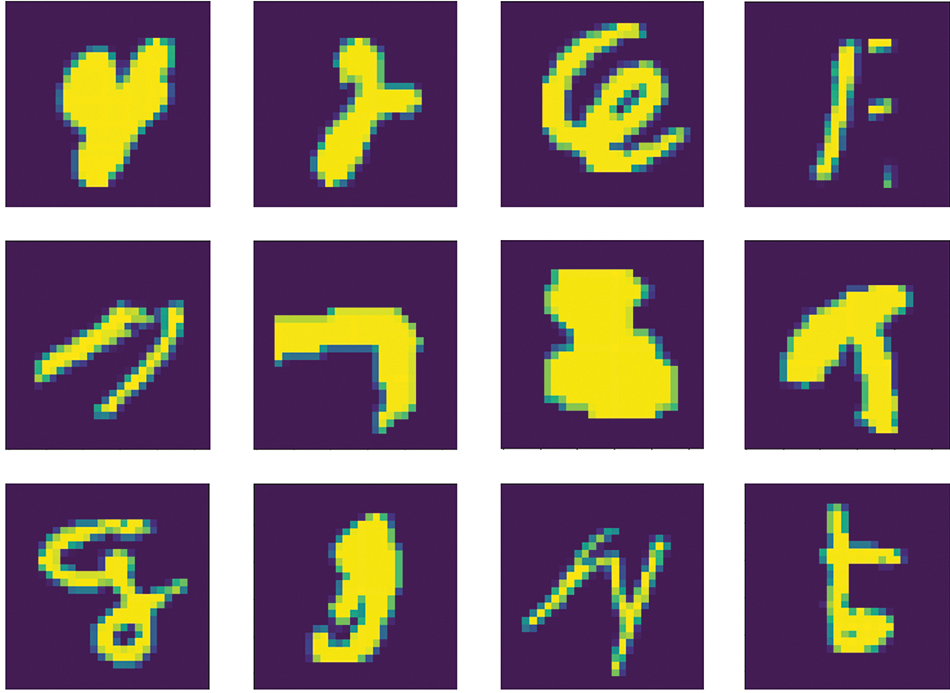
\includegraphics[width=\textwidth,height=0.7\textheight,keepaspectratio]{../../images/ch05/weird_mnist.84598aa0.png}
            \caption{Các ảnh bị nhiễu nặng trong tập MNIST}
        \end{figure}
    \end{columns}
\end{frame}

\begin{frame}{Dữ liệu bị gán nhãn sai (Mislabeled Data)}
    \begin{columns}
        \column{0.5\textwidth}
        \begin{itemize}
            \item Do sai sót chủ quan của con người (Human Error), một số dữ liệu có thể bị gán nhãn (label) hoàn toàn sai.
            \item Ví dụ: Rõ ràng là số 4 nhưng lại gán nhãn là số 9 trong tập MNIST.
            \item Nếu mô hình cố gắng uốn cong ranh giới quyết định (decision boundary) để "chữa" lại những nhãn sai này, nó sẽ nhận diện sai hàng loạt các hình số 4 tương tự trong tương lai.
        \end{itemize}
        
        \column{0.5\textwidth}
        \begin{figure}
            \centering
            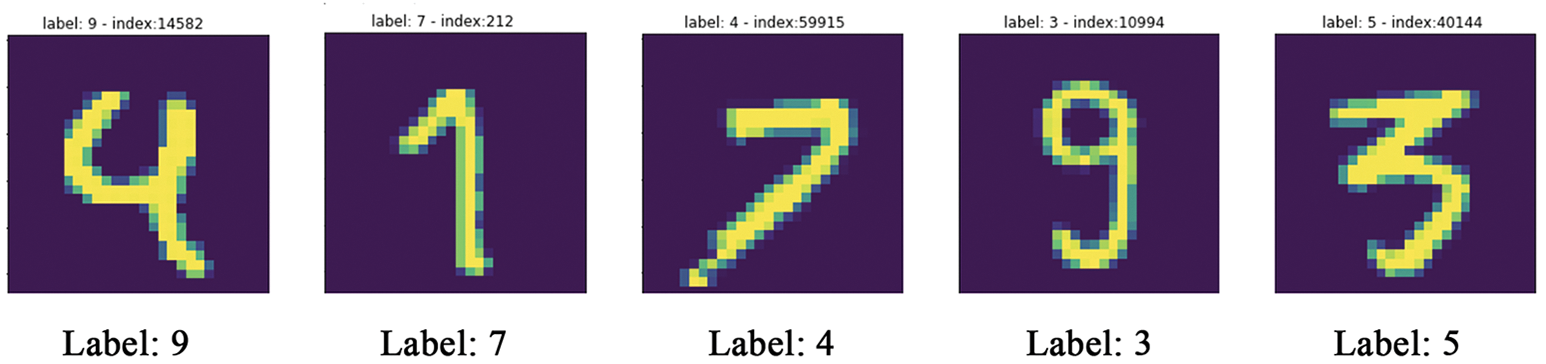
\includegraphics[width=\textwidth,height=0.7\textheight,keepaspectratio]{../../images/ch05/mislabeled_mnist.e7a71e65.png}
            \caption{Dữ liệu gán nhãn sai trong MNIST}
        \end{figure}
    \end{columns}
\end{frame}

\begin{frame}{Sự phình to của Kênh Nhiễu (Noise Channels)}
    \begin{columns}
        \column{0.5\textwidth}
        \begin{itemize}
            \item Thí nghiệm: Thêm một số ma trận toàn nhiễu trắng (white noise) hoặc toàn số 0 nối thêm vào dữ liệu MNIST ban đầu.
            \item Kết quả: Kể cả khi dữ liệu MNIST hợp lệ vẫn nguyên vẹn, mạng bị phân tâm bởi kênh nhiễu.
            \item Validation Accuracy của bộ dữ liệu chứa Noise Channels giảm rõ rệt. Lý do: Mô hình vô tình tìm ra các mẫu (patterns) ngẫu nhiên giả mạo trong tập nhiễu và sử dụng chúng để ra quyết định $\rightarrow$ Suy giảm Generalization.
        \end{itemize}
        
        \column{0.5\textwidth}
        \begin{figure}
            \centering
            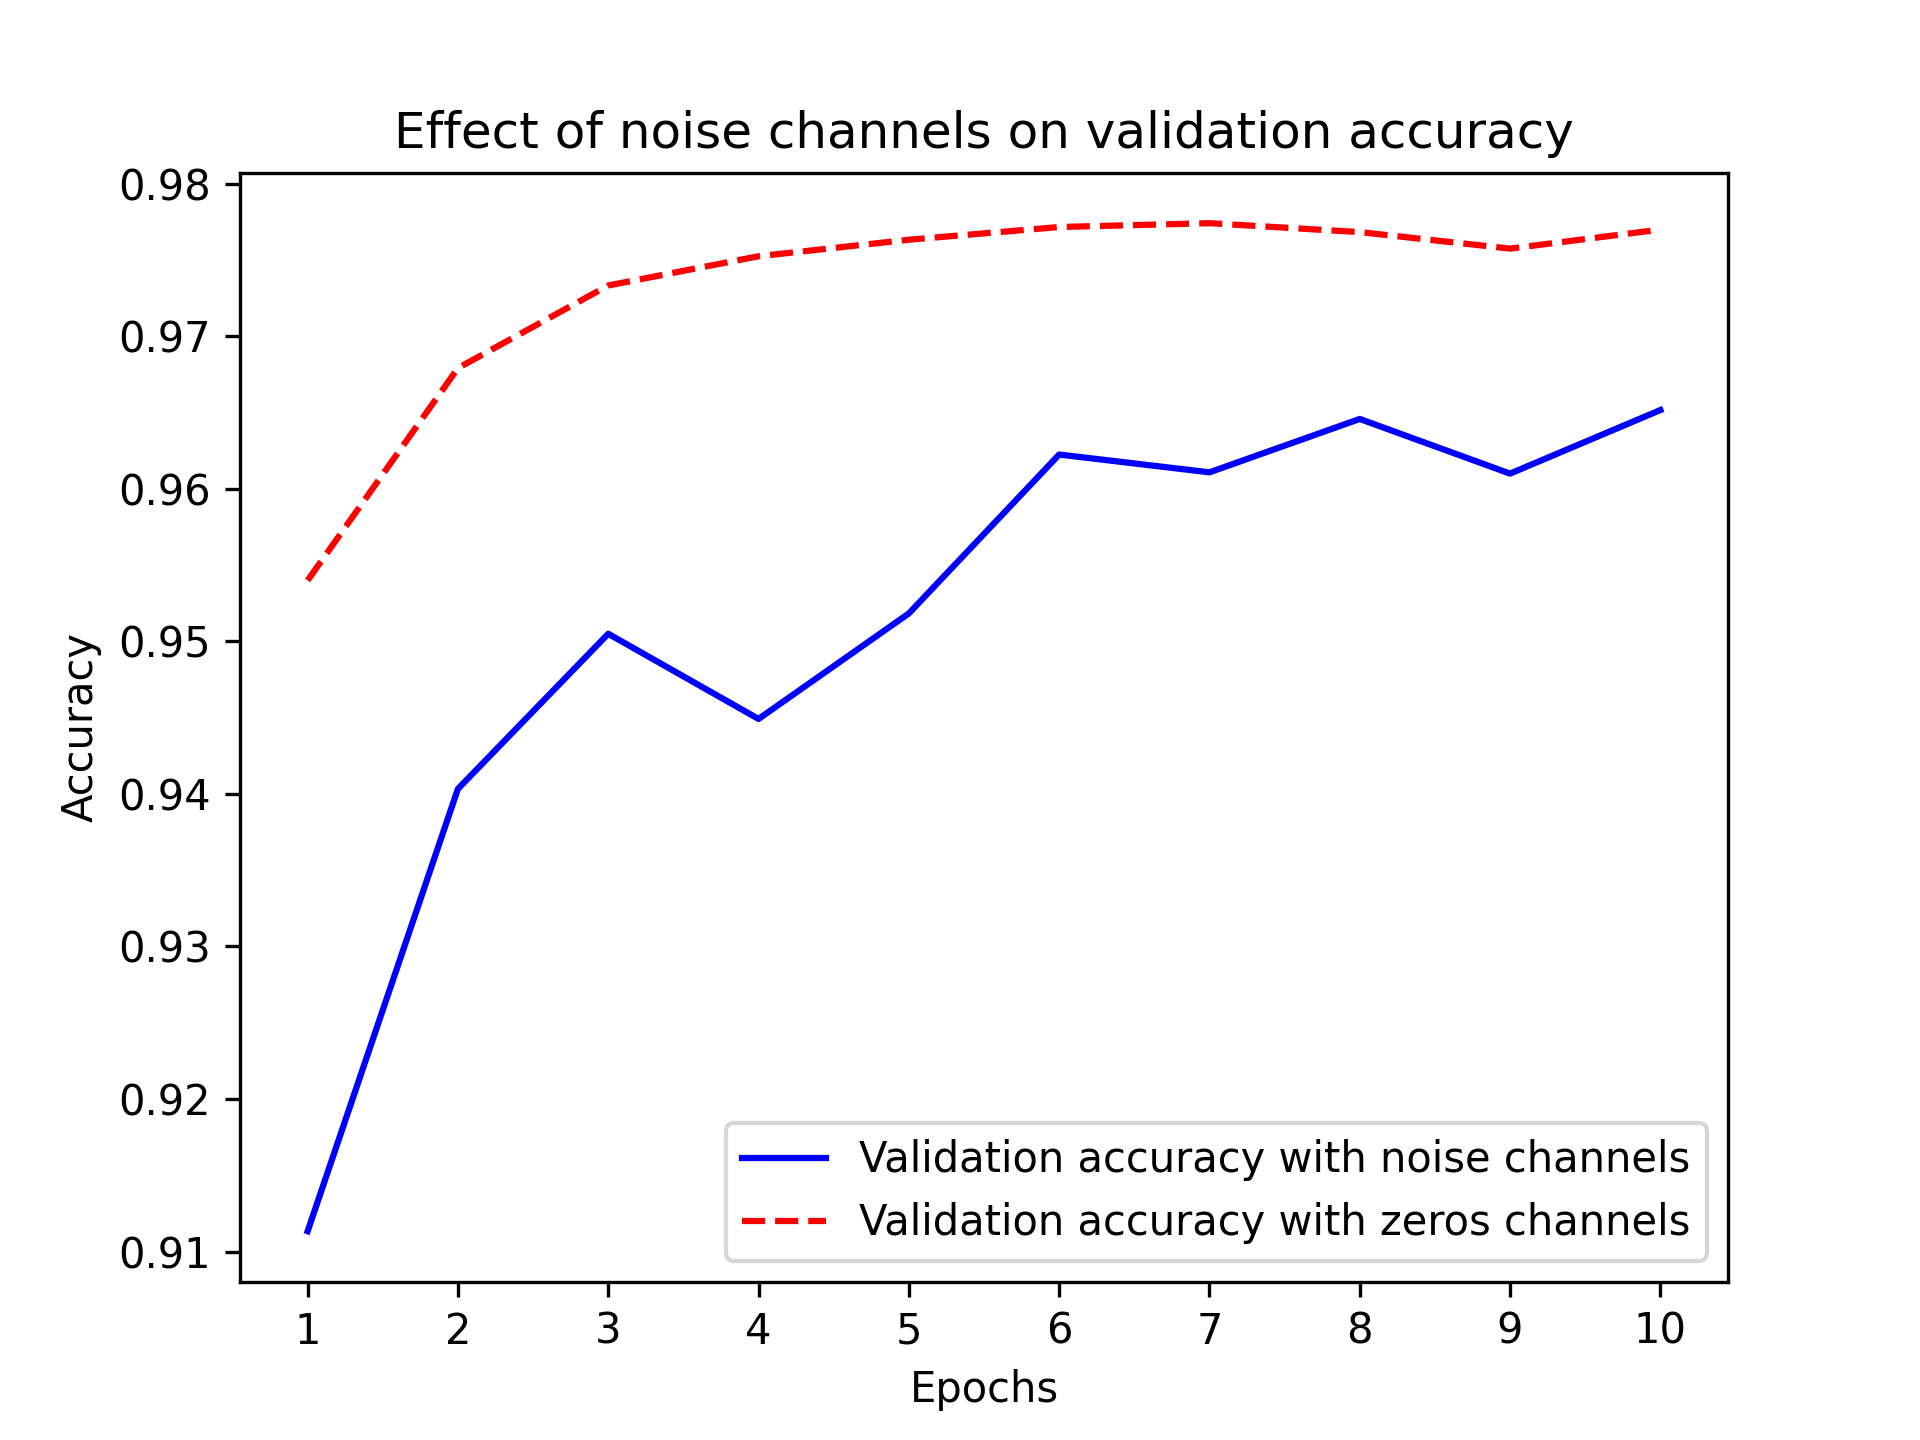
\includegraphics[width=\textwidth,height=0.7\textheight,keepaspectratio]{../../images/ch05/mnist_with_added_noise_channels_or_zeros_channels.0d1878dc.png}
            \caption{Tác động của kênh nhiễu đến Accuracy}
        \end{figure}
    \end{columns}
\end{frame}

\begin{frame}{Ngoại lai (Outliers) và Sự quá khớp}
    \begin{columns}
        \column{0.5\textwidth}
        \begin{itemize}
            \item Các điểm nhiễu thường đóng vai trò là "Ngoại lai" (Outliers), tức là các điểm dữ liệu nằm lạc lõng giữa quần thể lớp khác.
            \item Việc Gradient Descent nỗ lực cực độ để phân loại đúng 100\% tập huấn luyện sẽ ép đường ranh giới quyết định vươn xa ra ngoài để bọc lấy outlier.
            \item Hậu quả: Ranh giới quyết định trở nên góc cạnh thay vì là một đường cong mượt mà, bao quát.
        \end{itemize}
        
        \column{0.5\textwidth}
        \begin{figure}
            \centering
            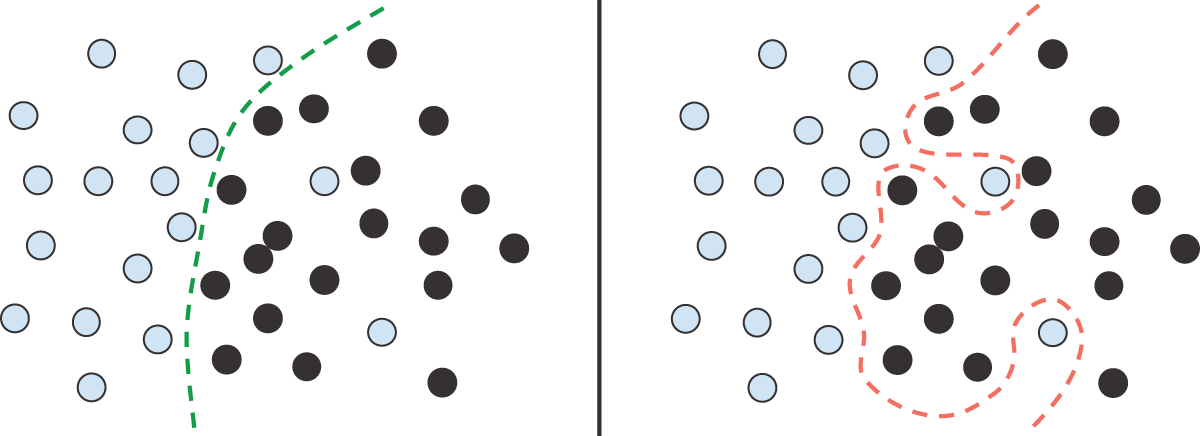
\includegraphics[width=\textwidth,height=0.7\textheight,keepaspectratio]{../../images/ch05/outliers_and_overfitting.919c6421.png}
            \caption{Robust fit (trái) vs. Overfitting ngoại lai (phải)}
        \end{figure}
    \end{columns}
\end{frame}

\begin{frame}{Đặc trưng mơ hồ (Ambiguous features)}
    \begin{columns}
        \column{0.5\textwidth}
        \begin{itemize}
            \item Đôi khi ranh giới giữa hai nhóm dữ liệu có vùng giao thoa. Tại vùng này, một dữ liệu có xác suất 50\% thuộc lớp A và 50\% thuộc lớp B (Uncertainty).
            \item Thay vì vạch một đường thẳng cắt đôi đám giao thoa mang tính chất thống kê này, Overfitting sẽ biến đường biên thành hình răng cưa uốn éo cố phân chia tách bạch.
            \item Khắc phục: Phải cho phép mô hình phạm lỗi trên tập Train (Training Loss không bao giờ bằng 0).
        \end{itemize}
        
        \column{0.5\textwidth}
        \begin{figure}
            \centering
            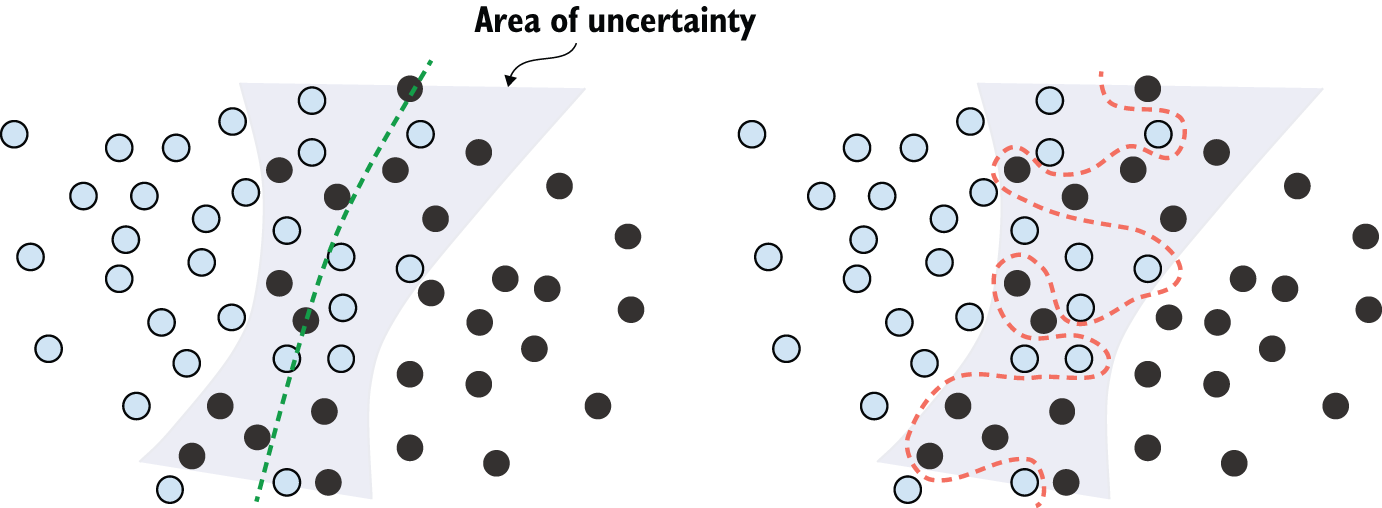
\includegraphics[width=\textwidth,height=0.7\textheight,keepaspectratio]{../../images/ch05/overfitting_with_uncertainty.7eace2a5.png}
            \caption{Overfitting trên vùng dữ liệu bất định}
        \end{figure}
    \end{columns}
\end{frame}

\section{3. Các phương pháp Đánh giá Mô hình}

\begin{frame}{Chia 3 tập: Train, Validation và Test}
    \begin{itemize}
        \item Tại sao không chỉ có 2 tập Train và Test?
        \item Quá trình huấn luyện không chỉ là điều chỉnh "Tham số" (Weights/Biases) qua Gradient Descent mà còn là điều chỉnh "Siêu tham số" (Hyperparameters - số lớp ẩn, số nơ-ron, learning rate...).
        \item Chúng ta dò tìm các cấu hình siêu tham số này để cải thiện điểm số trên tập Validation.
        \item \textbf{Information Leak:} Việc liên tục dùng tập Validation làm la bàn để tối ưu siêu tham số sẽ khiến mô hình gián tiếp "học lỏm" cấu trúc tập Validation $\rightarrow$ Overfit trên chính Validation.
        \item Do đó, ta bắt buộc phải có tập thứ 3: \textbf{Tập Test} (Hoàn toàn mới, chỉ chạy đúng 1 lần trước khi đưa ứng dụng vào thực tế).
    \end{itemize}
\end{frame}

\begin{frame}{Tách tập Validation đơn giản (Hold-out Validation)}
    \begin{columns}
        \column{0.5\textwidth}
        \begin{itemize}
            \item Xáo trộn dữ liệu (Shuffle) và tách một phần cố định (vd: 20\%) từ tập Training để làm tập Validation.
            \item Phương pháp này rất nhanh gọn, thường dùng khi khối lượng dữ liệu khổng lồ (hàng trăm ngàn điểm dữ liệu).
            \item Nhược điểm: Nếu dữ liệu ít, tập Validation sẽ không mang tính đại diện thống kê cho toàn bộ phân phối, dẫn tới sai số đánh giá lớn khi đổi seed chia tách.
        \end{itemize}
        
        \column{0.5\textwidth}
        \begin{figure}
            \centering
            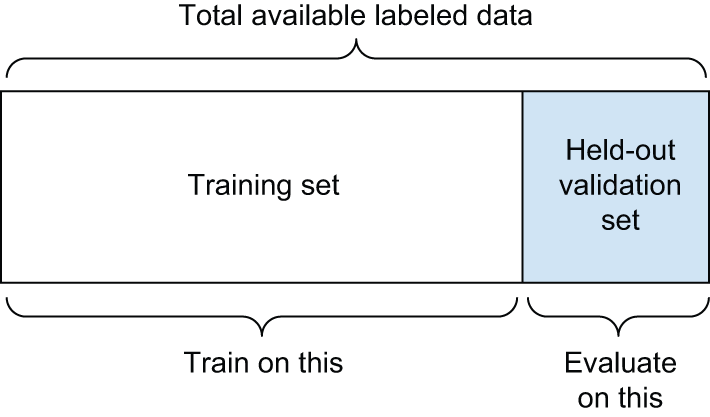
\includegraphics[width=\textwidth,height=0.7\textheight,keepaspectratio]{../../images/ch05/holdout_validation.55d20cbc.png}
            \caption{Quy trình Hold-out Validation}
        \end{figure}
    \end{columns}
\end{frame}

\begin{frame}[fragile]{Mã nguồn: Hold-out Validation}
\begin{lstlisting}[language=Python]
import numpy as np

num_val_samples = 10000
np.random.shuffle(data) # Xao tron ngau nhien

# Tach 10k mau lam Validation
val_data = data[:num_val_samples]
train_data = data[num_val_samples:]

model = get_model()
model.fit(train_data, epochs=20)
val_score = model.evaluate(val_data)

# Sau khi dieu chinh hyperparameter thanh cong, 
# ta huan luyen lai 1 mo hinh tren toan bo Train + Validation
model = get_model()
model.fit(np.concatenate([train_data, val_data]), epochs=20)
test_score = model.evaluate(test_data)
\end{lstlisting}
\end{frame}

\begin{frame}{Đánh giá chéo K-Lần (K-Fold Validation)}
    \begin{columns}
        \column{0.5\textwidth}
        \begin{itemize}
            \item Khi dữ liệu cực kỳ thưa thớt, việc Hold-out 1/5 lượng dữ liệu sẽ làm lãng phí cơ hội học tập của mạng.
            \item \textbf{K-Fold Validation:} Chia dữ liệu thành K phần (Fold). Lặp lại K vòng huấn luyện khác nhau. Ở vòng $i$, lấy Fold $i$ làm Validation, gộp tất cả $K-1$ Fold còn lại làm Training.
            \item Điểm số sau cùng là giá trị trung bình của $K$ điểm số đánh giá. 
            \item Độ chính xác cao, nhưng chi phí tài nguyên gấp $K$ lần.
        \end{itemize}
        
        \column{0.5\textwidth}
        \begin{figure}
            \centering
            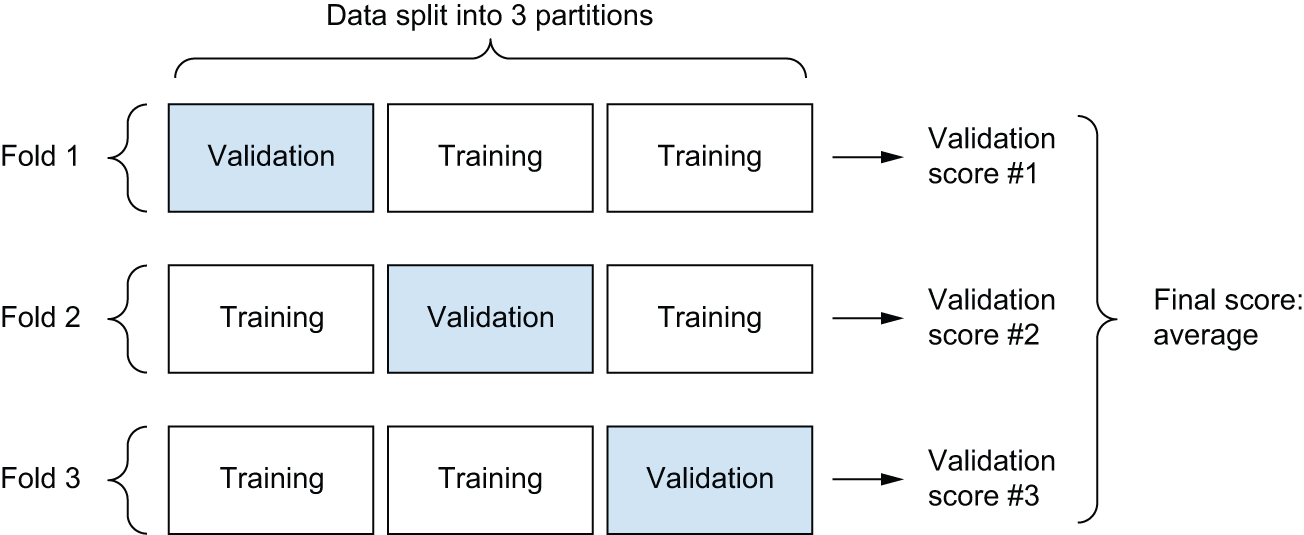
\includegraphics[width=\textwidth,height=0.7\textheight,keepaspectratio]{../../images/ch05/k_fold_validation.1fd60660.png}
            \caption{Quy trình K-Fold Validation (với K=3)}
        \end{figure}
    \end{columns}
\end{frame}

\begin{frame}[fragile]{Mã nguồn: K-Fold Validation}
\begin{lstlisting}[language=Python]
k = 4
num_val_samples = len(data) // k
val_scores = []

for fold in range(k):
    # Lay ra phan Validation rieng
    val_data = data[num_val_samples * fold : num_val_samples * (fold + 1)]
    
    # Gop phan dau va cuoi de tao thanh tap Train
    train_data = np.concatenate(
        [data[: num_val_samples * fold], data[num_val_samples * (fold + 1) :]], axis=0
    )
    
    model = get_model() # Khoi tao lai mo hinh moi hoan toan!
    model.fit(train_data, epochs=100, batch_size=16)
    score = model.evaluate(val_data)
    val_scores.append(score)

average_val_score = np.mean(val_scores) # Lay trung binh
\end{lstlisting}
\end{frame}

\section{4. Nâng cao chất lượng mô hình}

\begin{frame}[fragile]{Xử lý khi Validation Loss không chịu giảm}
    \begin{itemize}
        \item Đôi khi trong quá trình huấn luyện, Loss hoàn toàn không giảm và độ chính xác giữ nguyên ở ngưỡng Random Guess (chọn bừa).
        \item Điều này thường liên quan đến \textbf{Learning Rate} (Tốc độ học) đang quá cao hoặc quá thấp.
        \item Ví dụ: Tốc độ học khổng lồ `1.0` sẽ khiến các bước Gradient bay nhảy hỗn loạn trong không gian hàm mất mát.
    \end{itemize}
\begin{lstlisting}[language=Python]
# Tinh huong khien mo hinh "chet lam sang", Accuracy khong the tang
model.compile(
    optimizer=keras.optimizers.RMSprop(learning_rate=1.0),
    loss="sparse_categorical_crossentropy",
    metrics=["accuracy"],
)
\end{lstlisting}
\end{frame}

\begin{frame}[fragile]{Điều chỉnh Learning Rate và Batch Size}
    \begin{itemize}
        \item Khi hạ Learning Rate xuống mức tiêu chuẩn (ví dụ `1e-2`, `1e-3`), Loss sẽ bắt đầu giảm trơn tru.
        \item Nếu mạng vẫn không học, thử Tăng Batch Size. Lô dữ liệu lớn hơn sẽ tạo ra các vector đạo hàm ít nhiễu hơn, cung cấp định hướng chính xác hơn.
    \end{itemize}
\begin{lstlisting}[language=Python]
# Giam toc do hoc giup mo hinh hoi sinh
model.compile(
    optimizer=keras.optimizers.RMSprop(learning_rate=1e-2),
    loss="sparse_categorical_crossentropy",
    metrics=["accuracy"],
)
model.fit(train_images, train_labels, epochs=10, batch_size=128)
\end{lstlisting}
\end{frame}

\begin{frame}{Dung lượng Mô hình (Model Capacity) là gì?}
    \begin{itemize}
        \item Dung lượng của mạng nơ-ron tỷ lệ thuận với số lượng tham số (trọng số) mà nó sở hữu. Số lượng layer và số unit quyết định đại lượng này.
        \item \textbf{Dung lượng quá nhỏ:} Không đủ khả năng "ghi nhớ" các quy luật biểu diễn phi tuyến tính phức tạp $\rightarrow$ Underfitting.
        \item \textbf{Dung lượng quá lớn:} Quá dư thừa, mạng dễ dàng học vẹt (như một cuốn từ điển mapping từng input ra output) $\rightarrow$ Overfitting cực nhanh.
        \item Mục tiêu của người học sâu là thiết kế mạng có dung lượng vừa khít, có khả năng giảm loss tối đa nhưng trì hoãn việc overfit muộn nhất.
    \end{itemize}
\end{frame}

\begin{frame}{Khi Dung lượng Mô hình Không Đủ (Insufficient)}
    \begin{columns}
        \column{0.5\textwidth}
        \begin{itemize}
            \item Thử nghiệm dùng mạng hồi quy Logistic quá nhỏ (ví dụ cấu trúc nông chỉ xuất thẳng ra softmax) trên MNIST.
            \item Kết quả: Validation Loss không bao giờ xuống tới mức thấp mong muốn. Loss chững lại ở mức 0.26 và giữ nguyên (Stalled).
            \item Hiện tượng này xác nhận mạng không đủ sức mạnh để khái quát không gian giả thuyết phức tạp của hình ảnh.
        \end{itemize}
        
        \column{0.5\textwidth}
        \begin{figure}
            \centering
            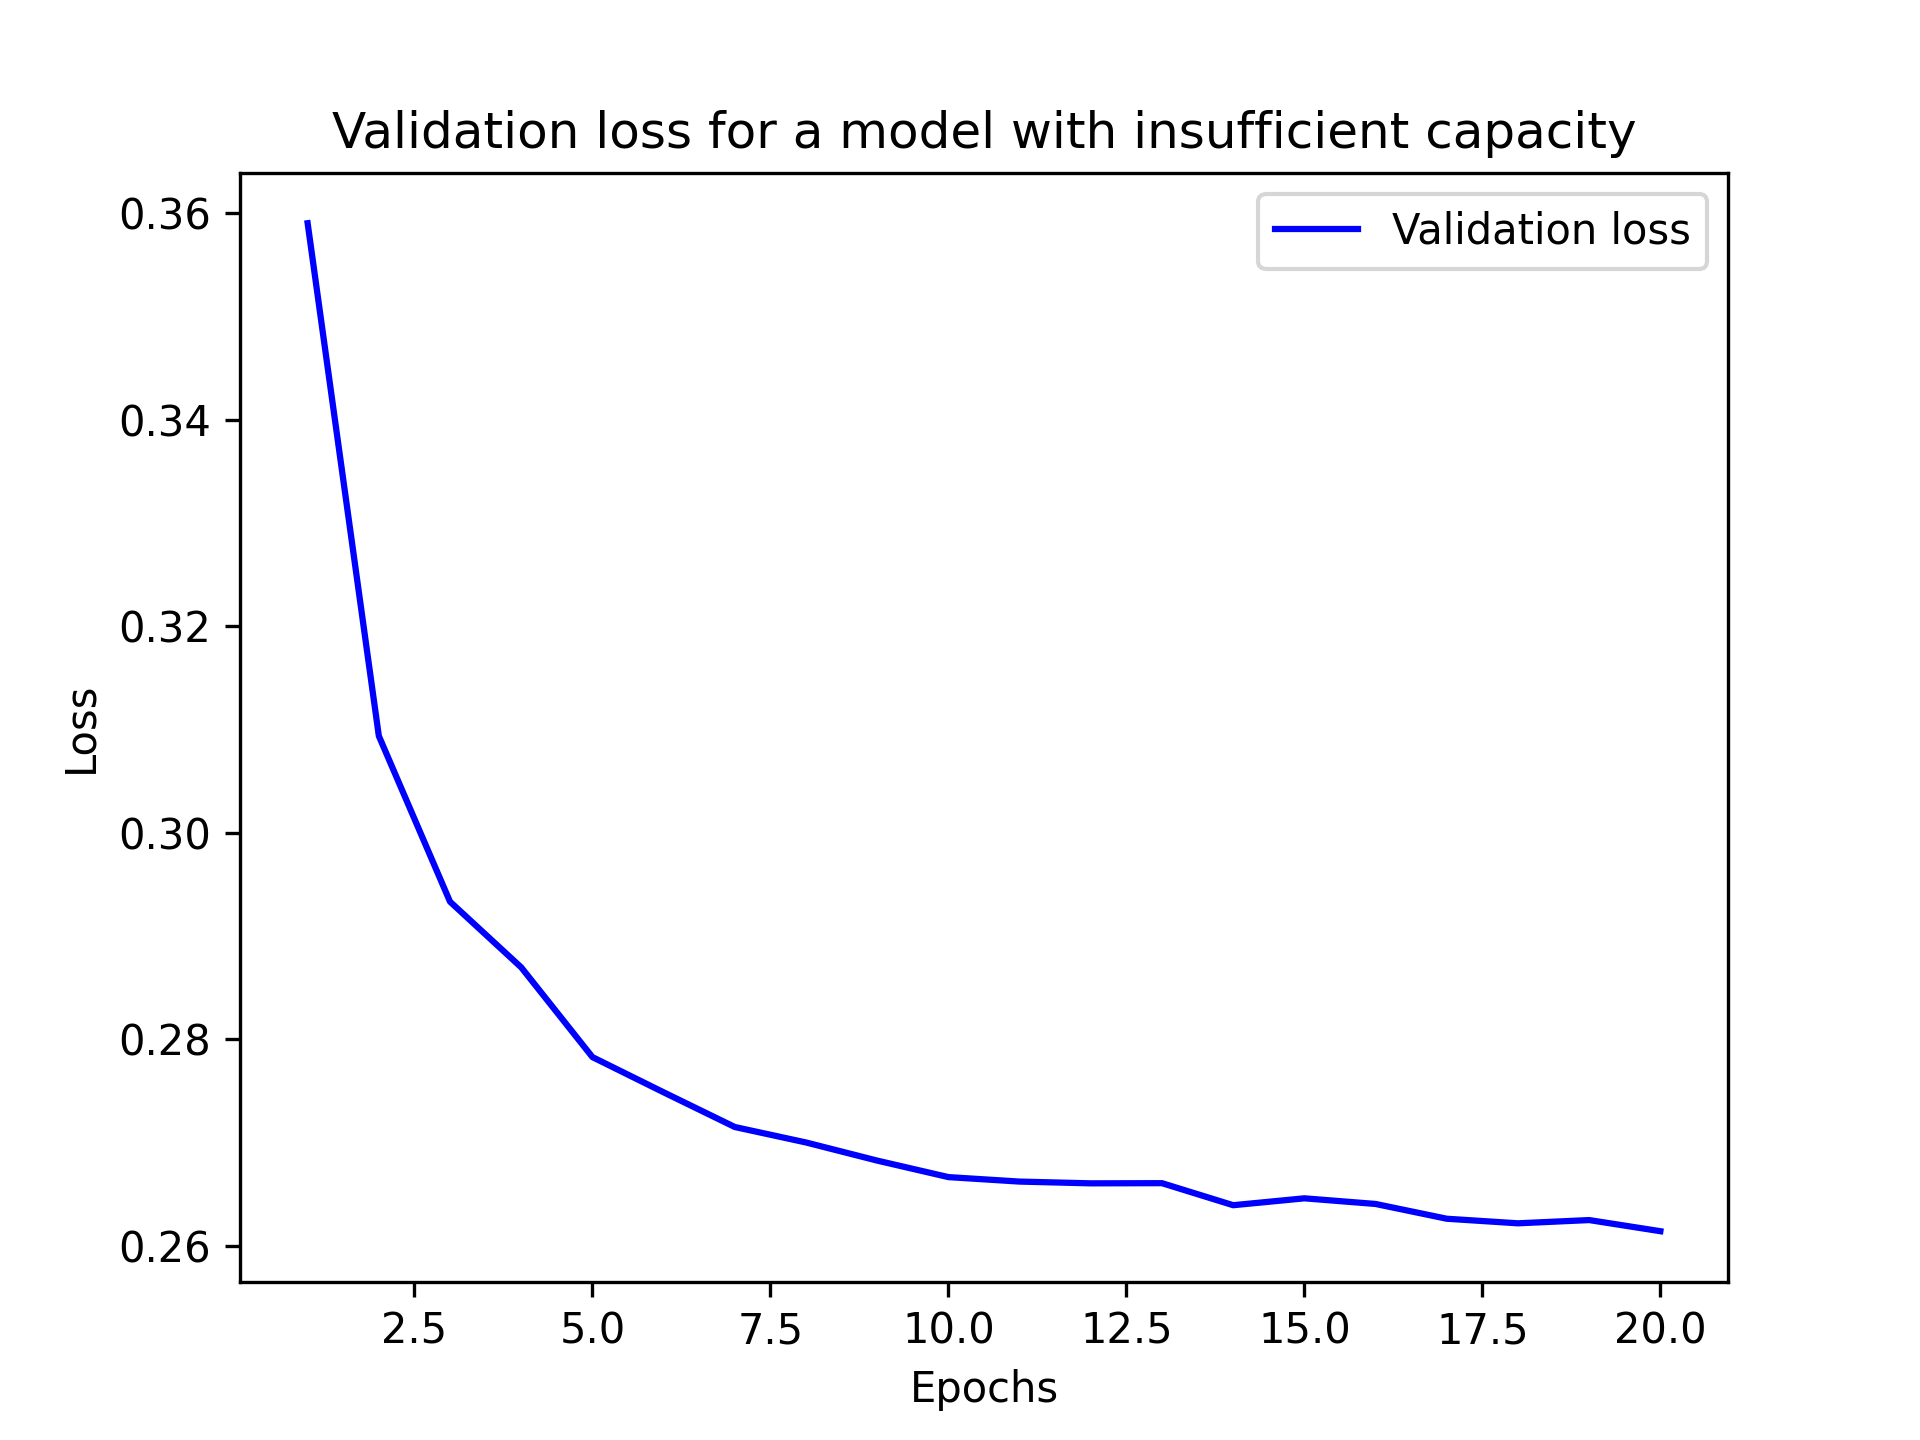
\includegraphics[width=\textwidth,height=0.7\textheight,keepaspectratio]{../../images/ch05/effect_of_insufficient_model_capacity_on_val_loss.3a003173.png}
            \caption{Loss khi Model Capacity quá yếu}
        \end{figure}
    \end{columns}
\end{frame}

\begin{frame}{Khi Dung lượng Mô hình Quá Lớn (Excessive)}
    \begin{columns}
        \column{0.5\textwidth}
        \begin{itemize}
            \item Thử nghiệm dùng mạng khổng lồ (3 lớp ẩn, mỗi lớp 2048 nơ-ron - hàng chục triệu tham số).
            \item Kết quả: Do sức mạnh học vẹt quá kinh khủng, nó nhớ toàn bộ tập Training trong vài giây. Validation Loss chạm đáy ngay tại Epoch 1, sau đó vọt lên mạnh mẽ.
            \item Đường Validation Loss cũng rất nhiễu (noise) chứng tỏ sự mất ổn định.
        \end{itemize}
        
        \column{0.5\textwidth}
        \begin{figure}
            \centering
            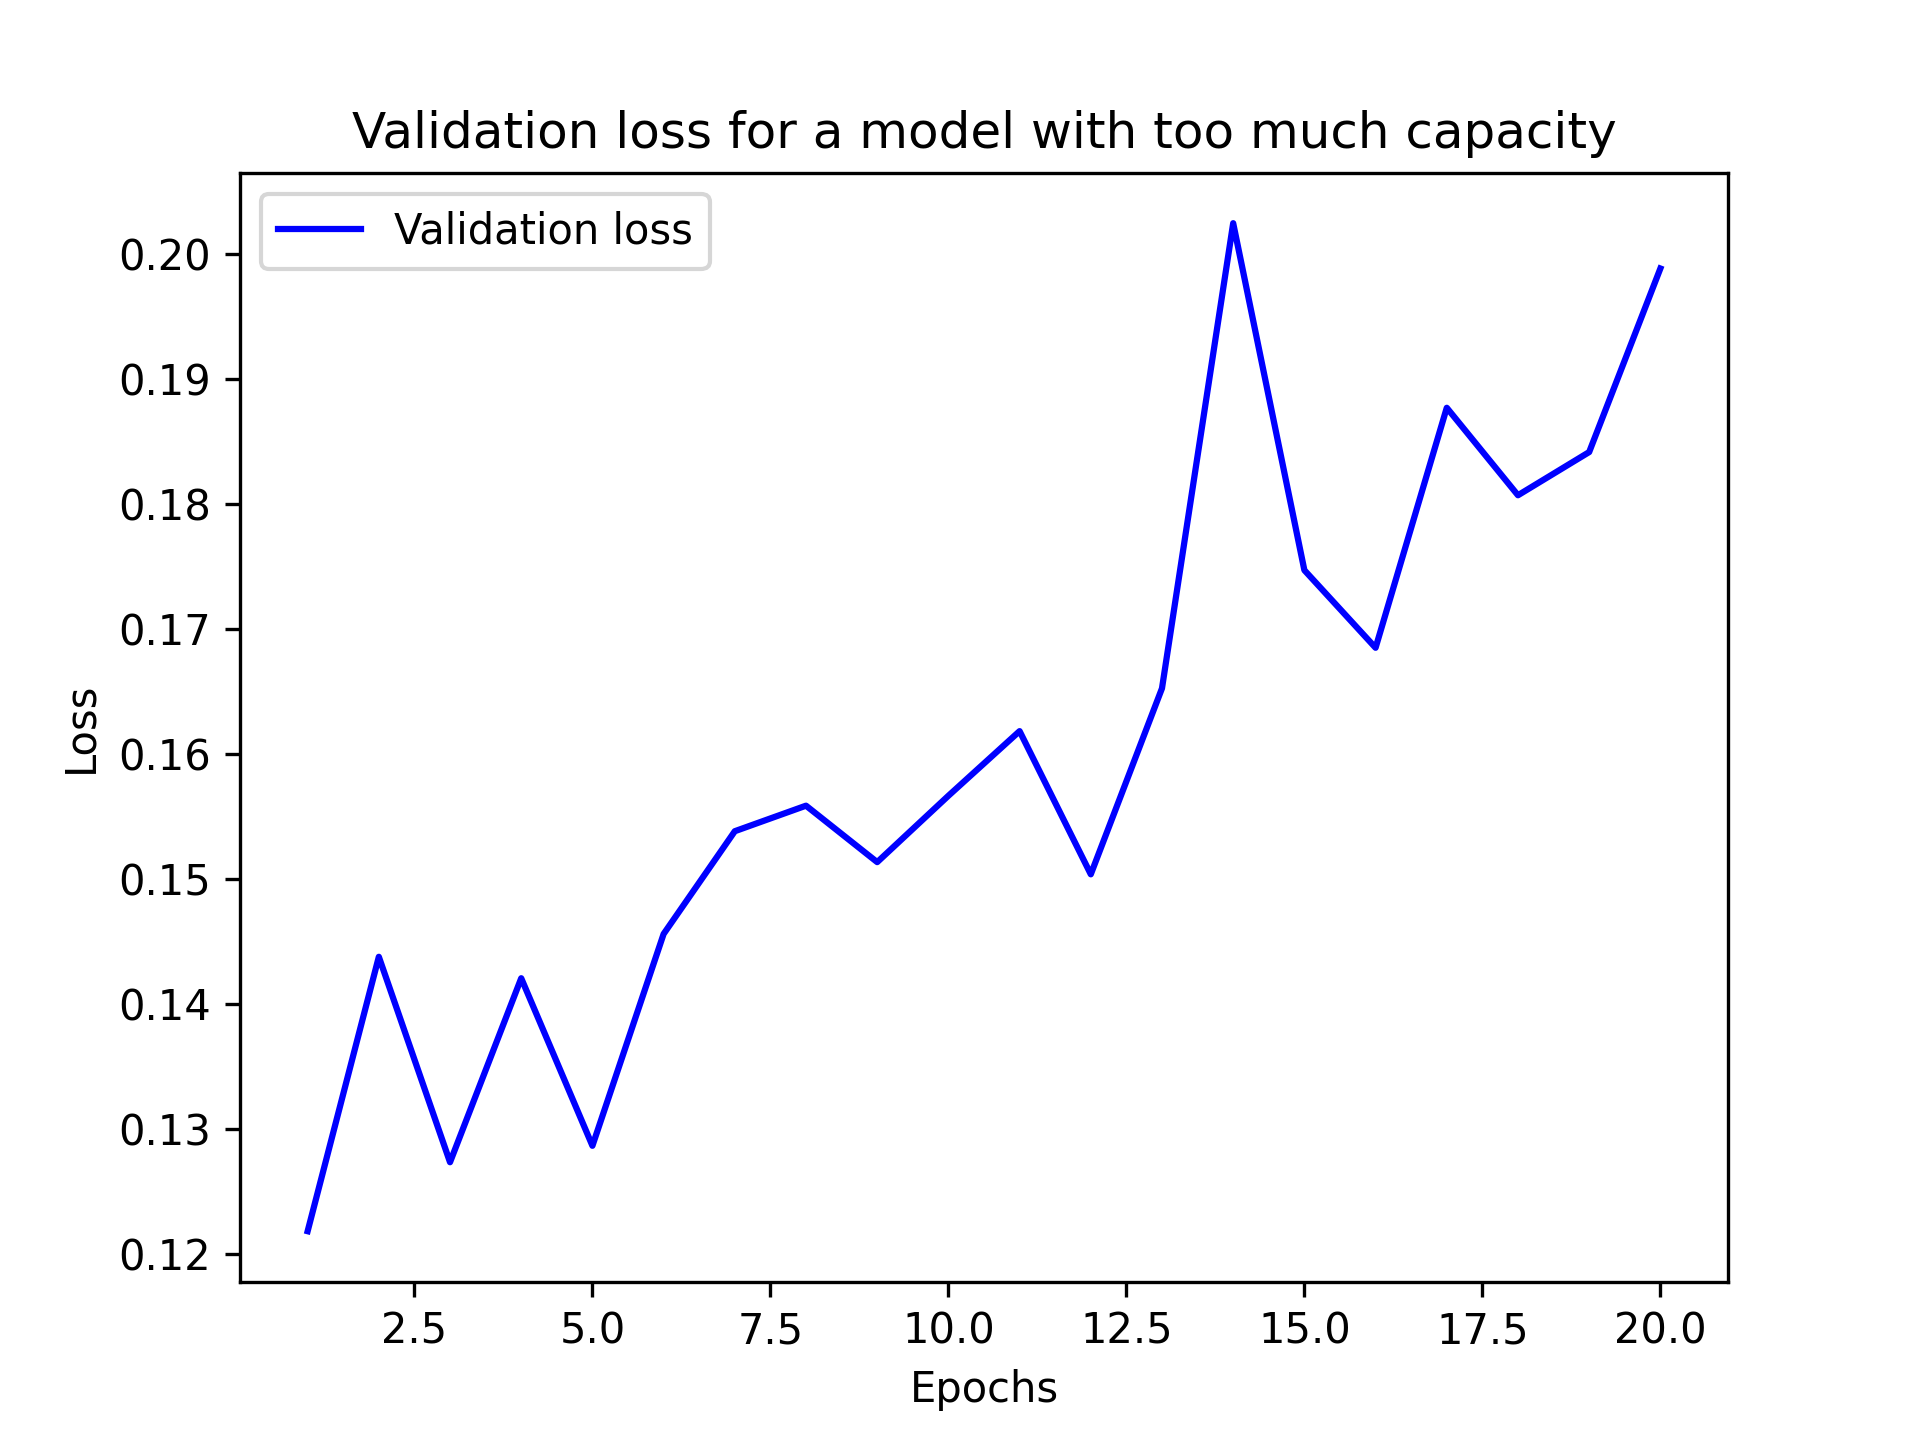
\includegraphics[width=\textwidth,height=0.7\textheight,keepaspectratio]{../../images/ch05/effect_of_excessive_model_capacity_on_val_loss.8defeb2b.png}
            \caption{Loss khi Model Capacity quá lớn}
        \end{figure}
    \end{columns}
\end{frame}

\begin{frame}{Dung lượng Mô hình Lý Tưởng (Correct Capacity)}
    \begin{columns}
        \column{0.5\textwidth}
        \begin{itemize}
            \item Mô hình có 2 lớp ẩn (mỗi lớp 128 units).
            \item Validation Loss giảm từ từ và duy trì ở mức tối thiểu trước khi bắt đầu có dấu hiệu tăng nhẹ ở epoch thứ 8.
            \item Đây là thiết kế kiến trúc (Architecture) cân bằng tuyệt vời giữa tối ưu hóa và khái quát hóa dữ liệu hình chữ số MNIST.
        \end{itemize}
        
        \column{0.5\textwidth}
        \begin{figure}
            \centering
            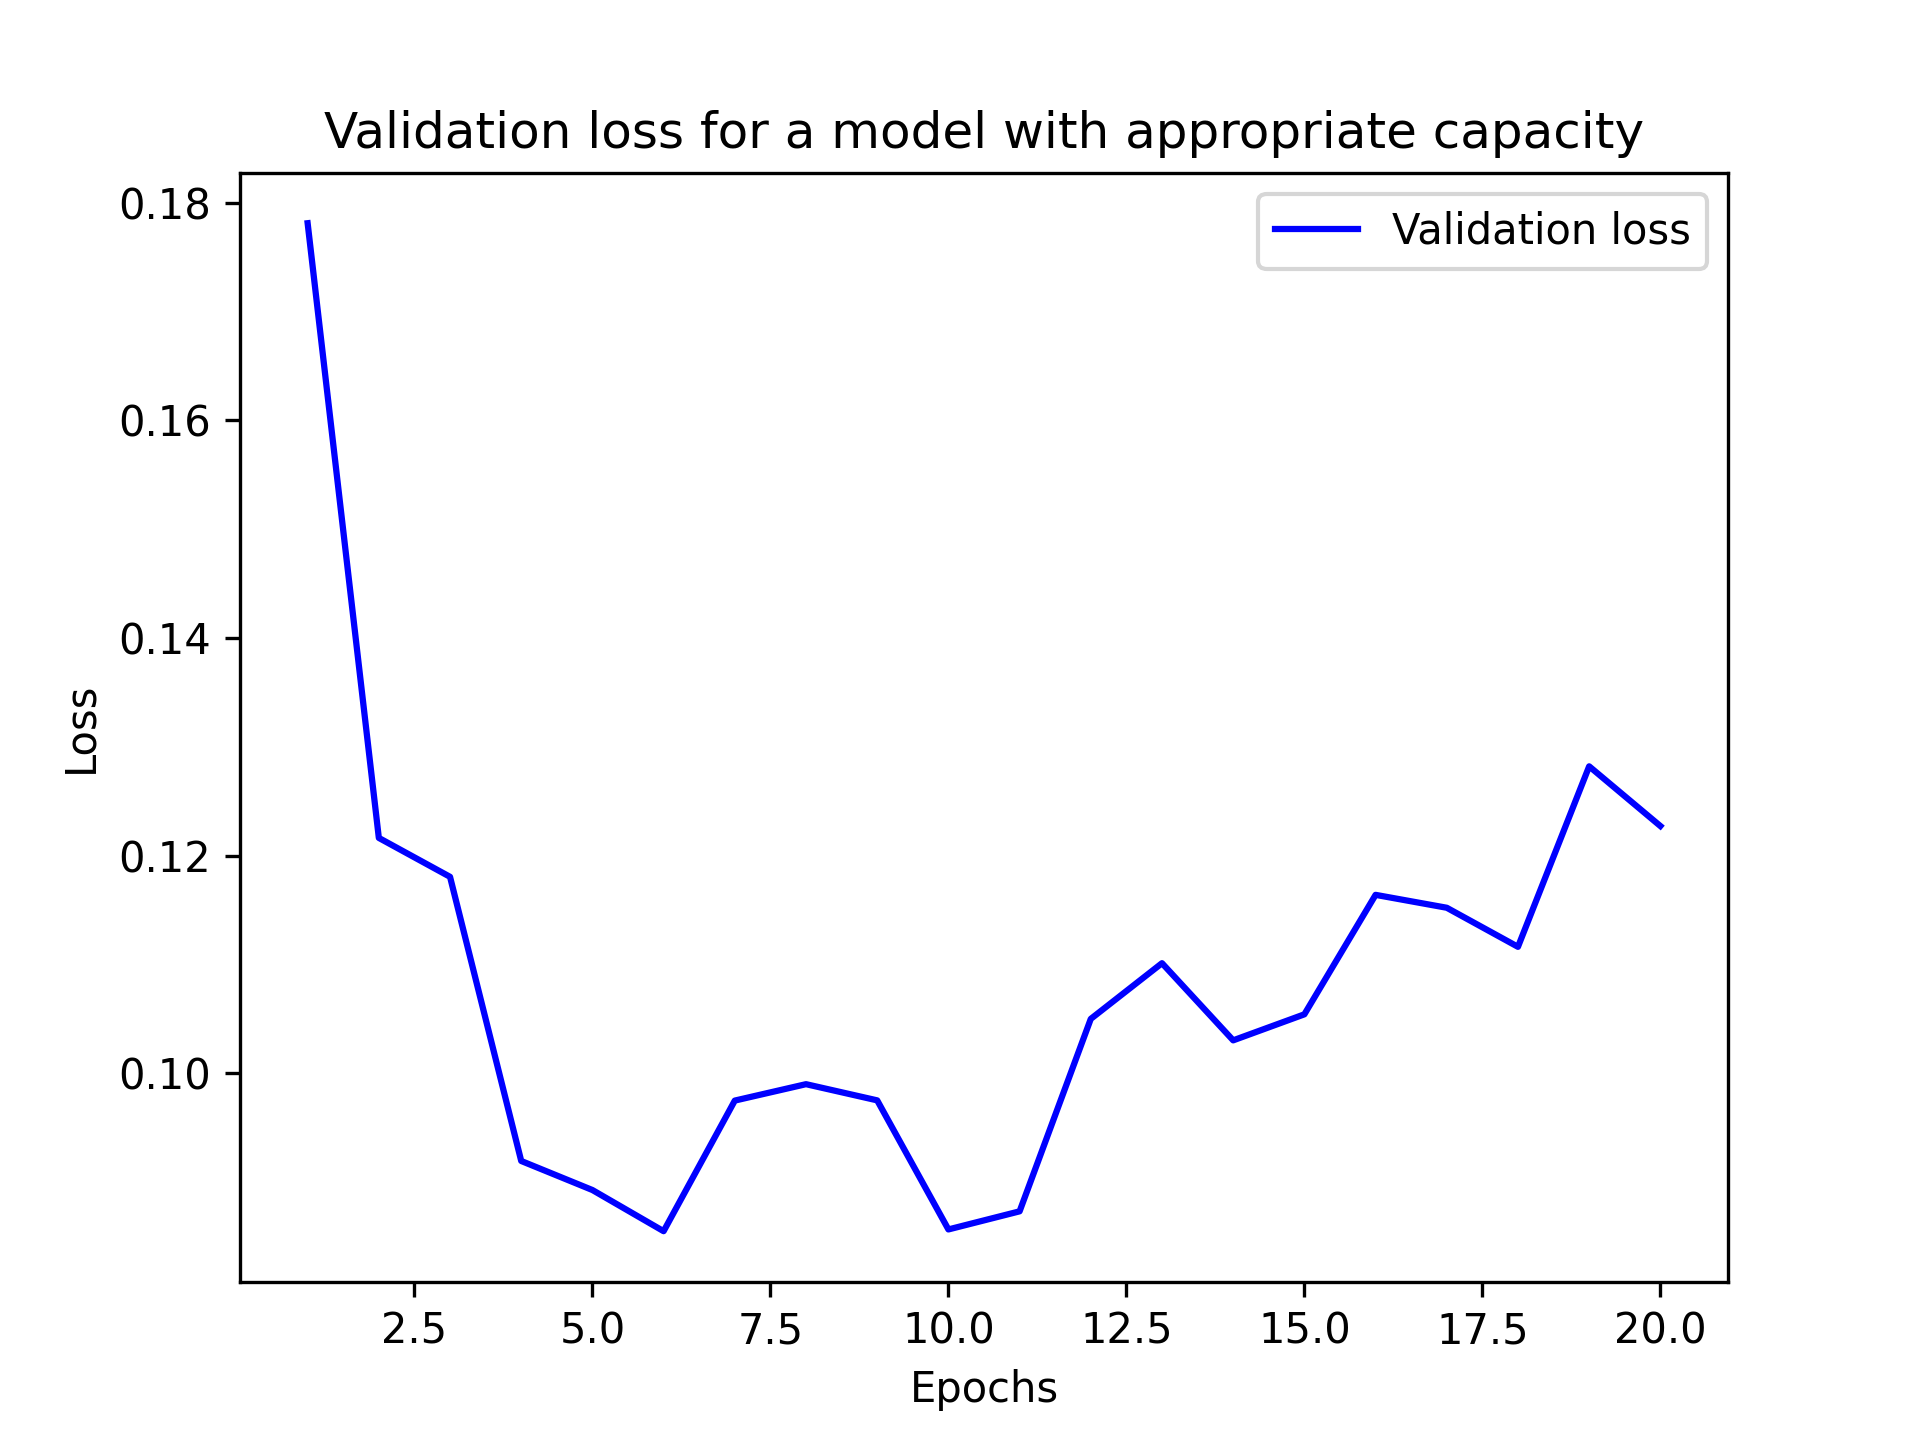
\includegraphics[width=\textwidth,height=0.7\textheight,keepaspectratio]{../../images/ch05/effect_of_correct_model_capacity_on_val_loss.1b765d5c.png}
            \caption{Loss khi Model Capacity phù hợp}
        \end{figure}
    \end{columns}
\end{frame}

\begin{frame}[fragile]{So sánh trên bài toán IMDB (Phân tích cảm xúc)}
    \begin{itemize}
        \item Mạng phân tích phim gốc ở Chương 4 sử dụng 2 lớp, 16 units.
        \item Hãy thử nghiệm giảm xuống còn 4 units, và tăng vọt lên 512 units.
    \end{itemize}
\begin{lstlisting}[language=Python]
# Mang IMDB goc (16 units)
model_base = keras.Sequential([
    layers.Dense(16, activation="relu"),
    layers.Dense(16, activation="relu"),
    layers.Dense(1, activation="sigmoid")
])

# Mang IMDB nho (4 units) -> Muc tieu giam thieu Overfitting
model_small = keras.Sequential([
    layers.Dense(4, activation="relu"),
    layers.Dense(4, activation="relu"),
    layers.Dense(1, activation="sigmoid")
])
\end{lstlisting}
\end{frame}


\begin{frame}{Trực quan: Mạng Gốc (16 units) vs Mạng Nhỏ Hơn (4 units)}
    \begin{columns}
        \column{0.5\textwidth}
        \begin{itemize}
            \item Đường có dấu chấm tròn (Dots) đại diện cho Mạng gốc 16 units.
            \item Đường đứt khúc (Solid/Crosses) đại diện cho Mạng nhỏ 4 units.
            \item Phân tích: Mạng nhỏ (Dung lượng thấp) phải mất nhiều epoch hơn (6 epoch) để bắt đầu có dấu hiệu tăng Validation Loss. Khi Overfit, đồ thị cũng dốc thoai thoải chậm hơn rất nhiều so với bản gốc.
            \item Kết luận: Giảm dung lượng mạng là kỹ thuật Regularization gốc rễ.
        \end{itemize}
        
        \column{0.5\textwidth}
        \begin{figure}
            \centering
            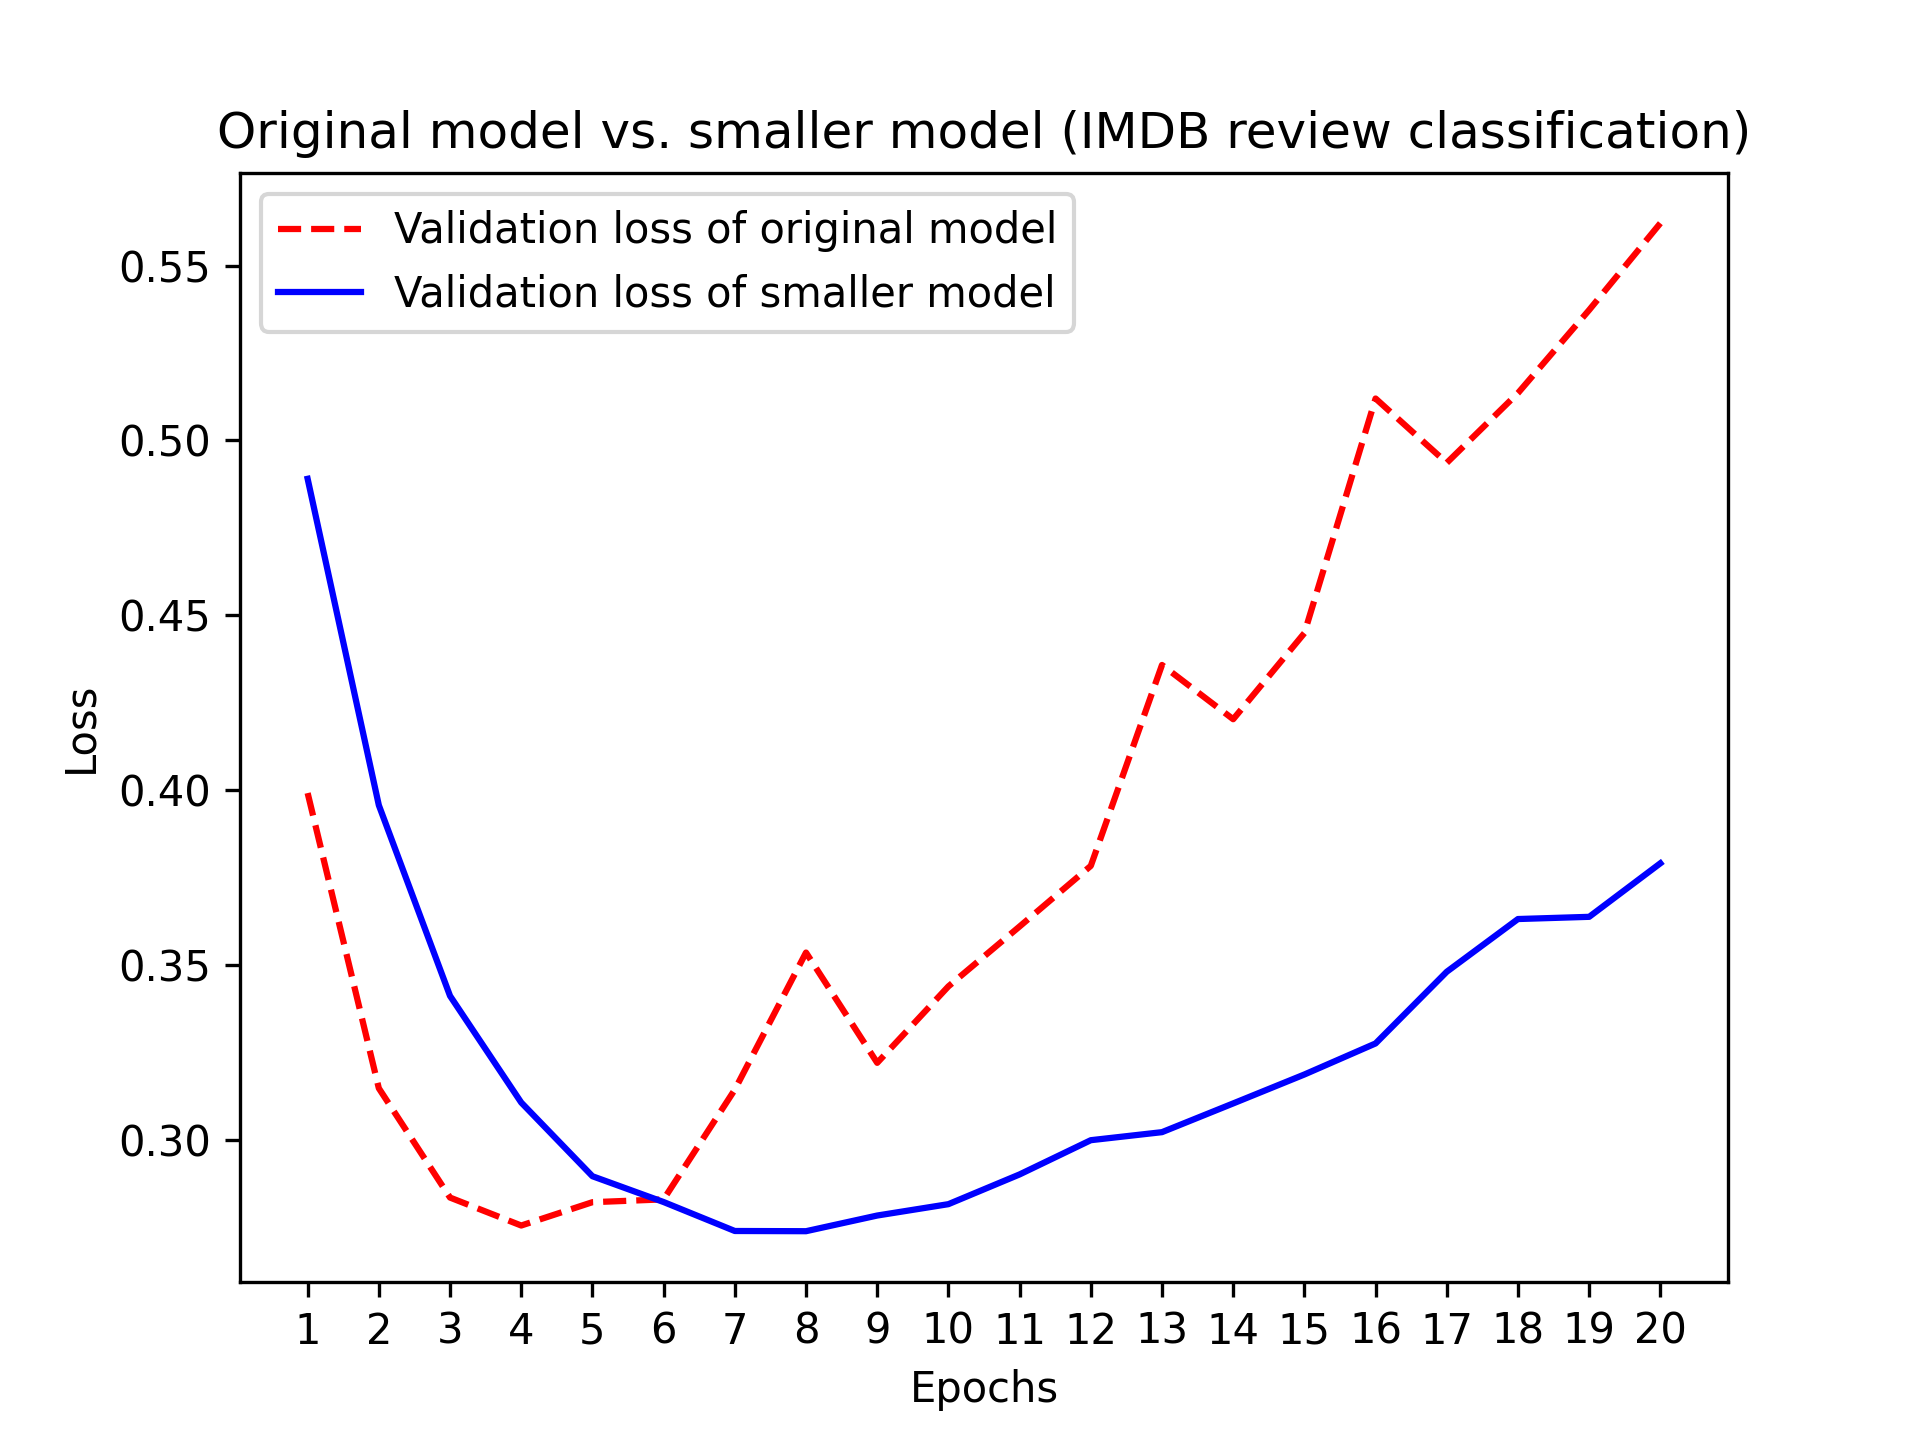
\includegraphics[width=\textwidth,height=0.7\textheight,keepaspectratio]{../../images/ch05/original_model_vs_smaller_model_imdb.906f7067.png}
            \caption{Mạng nhỏ (Crosses) vs Mạng gốc (Dots)}
        \end{figure}
    \end{columns}
\end{frame}

\begin{frame}{Trực quan: Mạng Gốc (16 units) vs Mạng Lớn Hơn (512 units)}
    \begin{columns}
        \column{0.5\textwidth}
        \begin{itemize}
            \item Đường có dấu chấm tròn (Dots) đại diện cho Mạng gốc 16 units.
            \item Đường đứt khúc đại diện cho Mạng 512 units.
            \item Phân tích: Mạng 512 units rơi vào tình trạng "Ghi nhớ thần tốc". Ngay từ epoch đầu tiên nó đã Overfit dữ dội và vọt lên rất cao, biên độ của Loss bị nhiễu lớn.
        \end{itemize}
        
        \column{0.5\textwidth}
        \begin{figure}
            \centering
            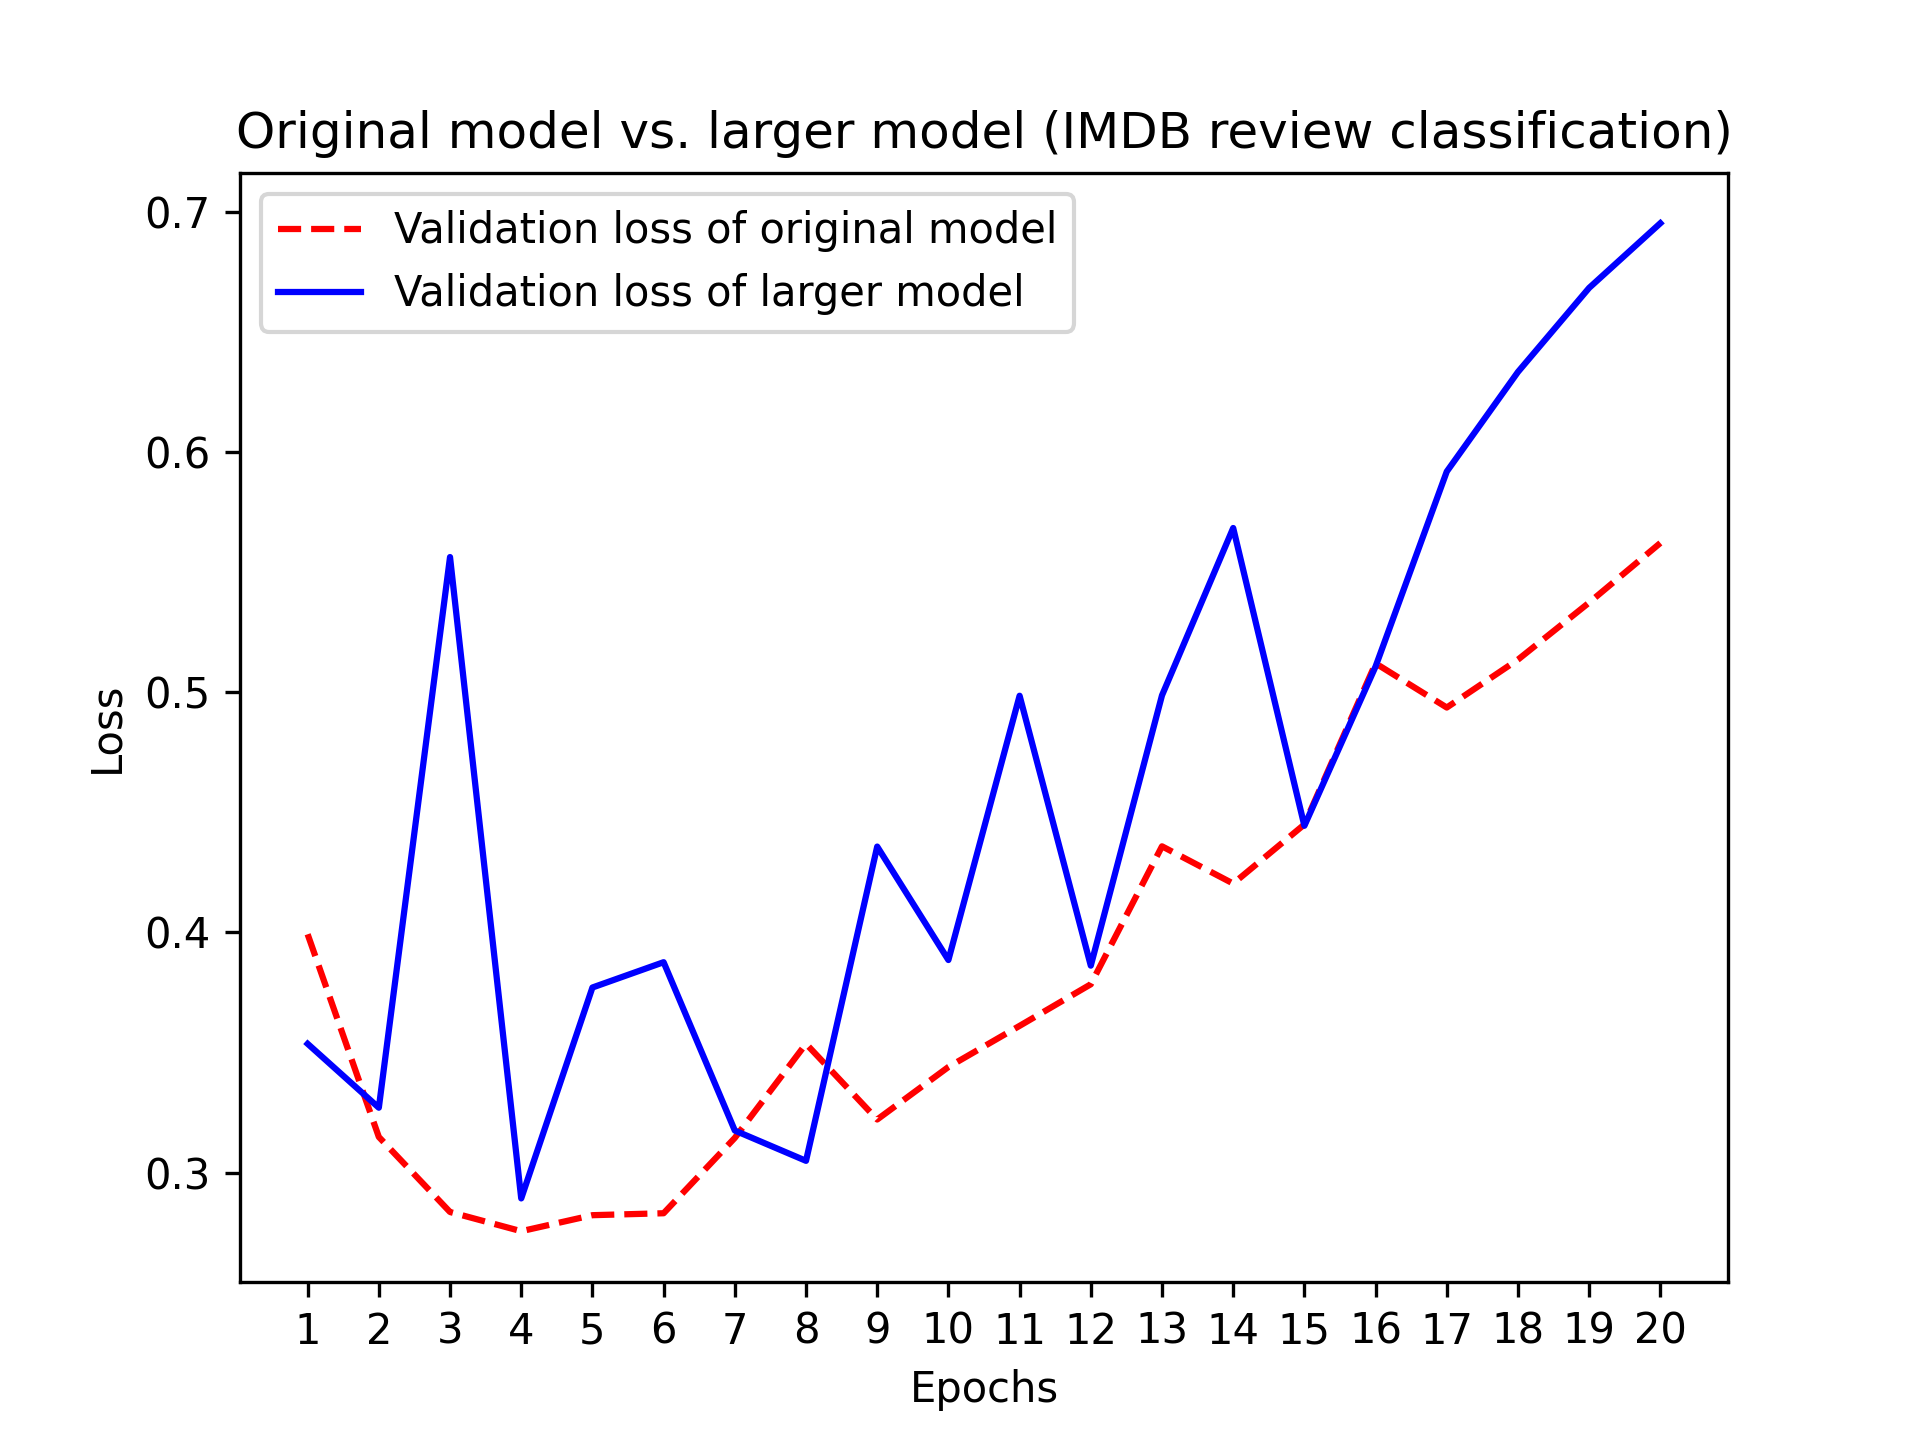
\includegraphics[width=\textwidth,height=0.7\textheight,keepaspectratio]{../../images/ch05/original_model_vs_larger_model_imdb.7d1bbc06.png}
            \caption{Mạng lớn (Crosses) vs Mạng gốc (Dots)}
        \end{figure}
    \end{columns}
\end{frame}

\section{5. Các Phương pháp Regularization chuyên sâu}

\begin{frame}[fragile]{Weight Regularization (Phạt Trọng Số L1 / L2)}
    \begin{itemize}
        \item Áp dụng nguyên lý Ockham's razor: Lời giải thích đơn giản hơn thường có xu hướng đúng. Một mô hình có các trọng số siêu nhỏ phân bố đều thì đơn giản hơn một mô hình chứa các trọng số khổng lồ bất thường.
        \item \textbf{L1 Regularization:} Thêm mức phạt tỷ lệ với trị tuyệt đối của trọng số $|W|$. Sẽ ép nhiều trọng số về đúng bằng $0$ (Tạo sự thưa thớt - Sparsity).
        \item \textbf{L2 Regularization (Weight Decay):} Thêm mức phạt tỷ lệ thuận với bình phương trọng số $W^2$. Ép trọng số nhỏ về tiệm cận $0$.
    \end{itemize}
\begin{lstlisting}[language=Python]
from keras.regularizers import l2, l1_l2

# Them tham so kernel_regularizer de tich hop Phat trong so
model = keras.Sequential([
    layers.Dense(16, kernel_regularizer=l2(0.002), activation="relu"),
    layers.Dense(16, kernel_regularizer=l2(0.002), activation="relu"),
    layers.Dense(1, activation="sigmoid")
])
\end{lstlisting}
\end{frame}

\begin{frame}{Hiệu quả của Phạt trọng số L2}
    \begin{columns}
        \column{0.5\textwidth}
        \begin{itemize}
            \item Tham số `l2(0.002)` sẽ cộng thêm $0.002 \times W^2$ vào hàm Loss gốc. Lưu ý, khoản phạt này chỉ tác động lúc Huấn luyện, tắt hoàn toàn lúc Kiểm tra.
            \item Biểu đồ cho thấy mạng dùng L2 (Crosses) duy trì Validation Loss ở mức an toàn và lâu overfit hơn đáng kể so với mạng không phạt.
            \item Thường được dùng tốt nhất trên các mô hình có kích cỡ bé và vừa.
        \end{itemize}
        
        \column{0.5\textwidth}
        \begin{figure}
            \centering
            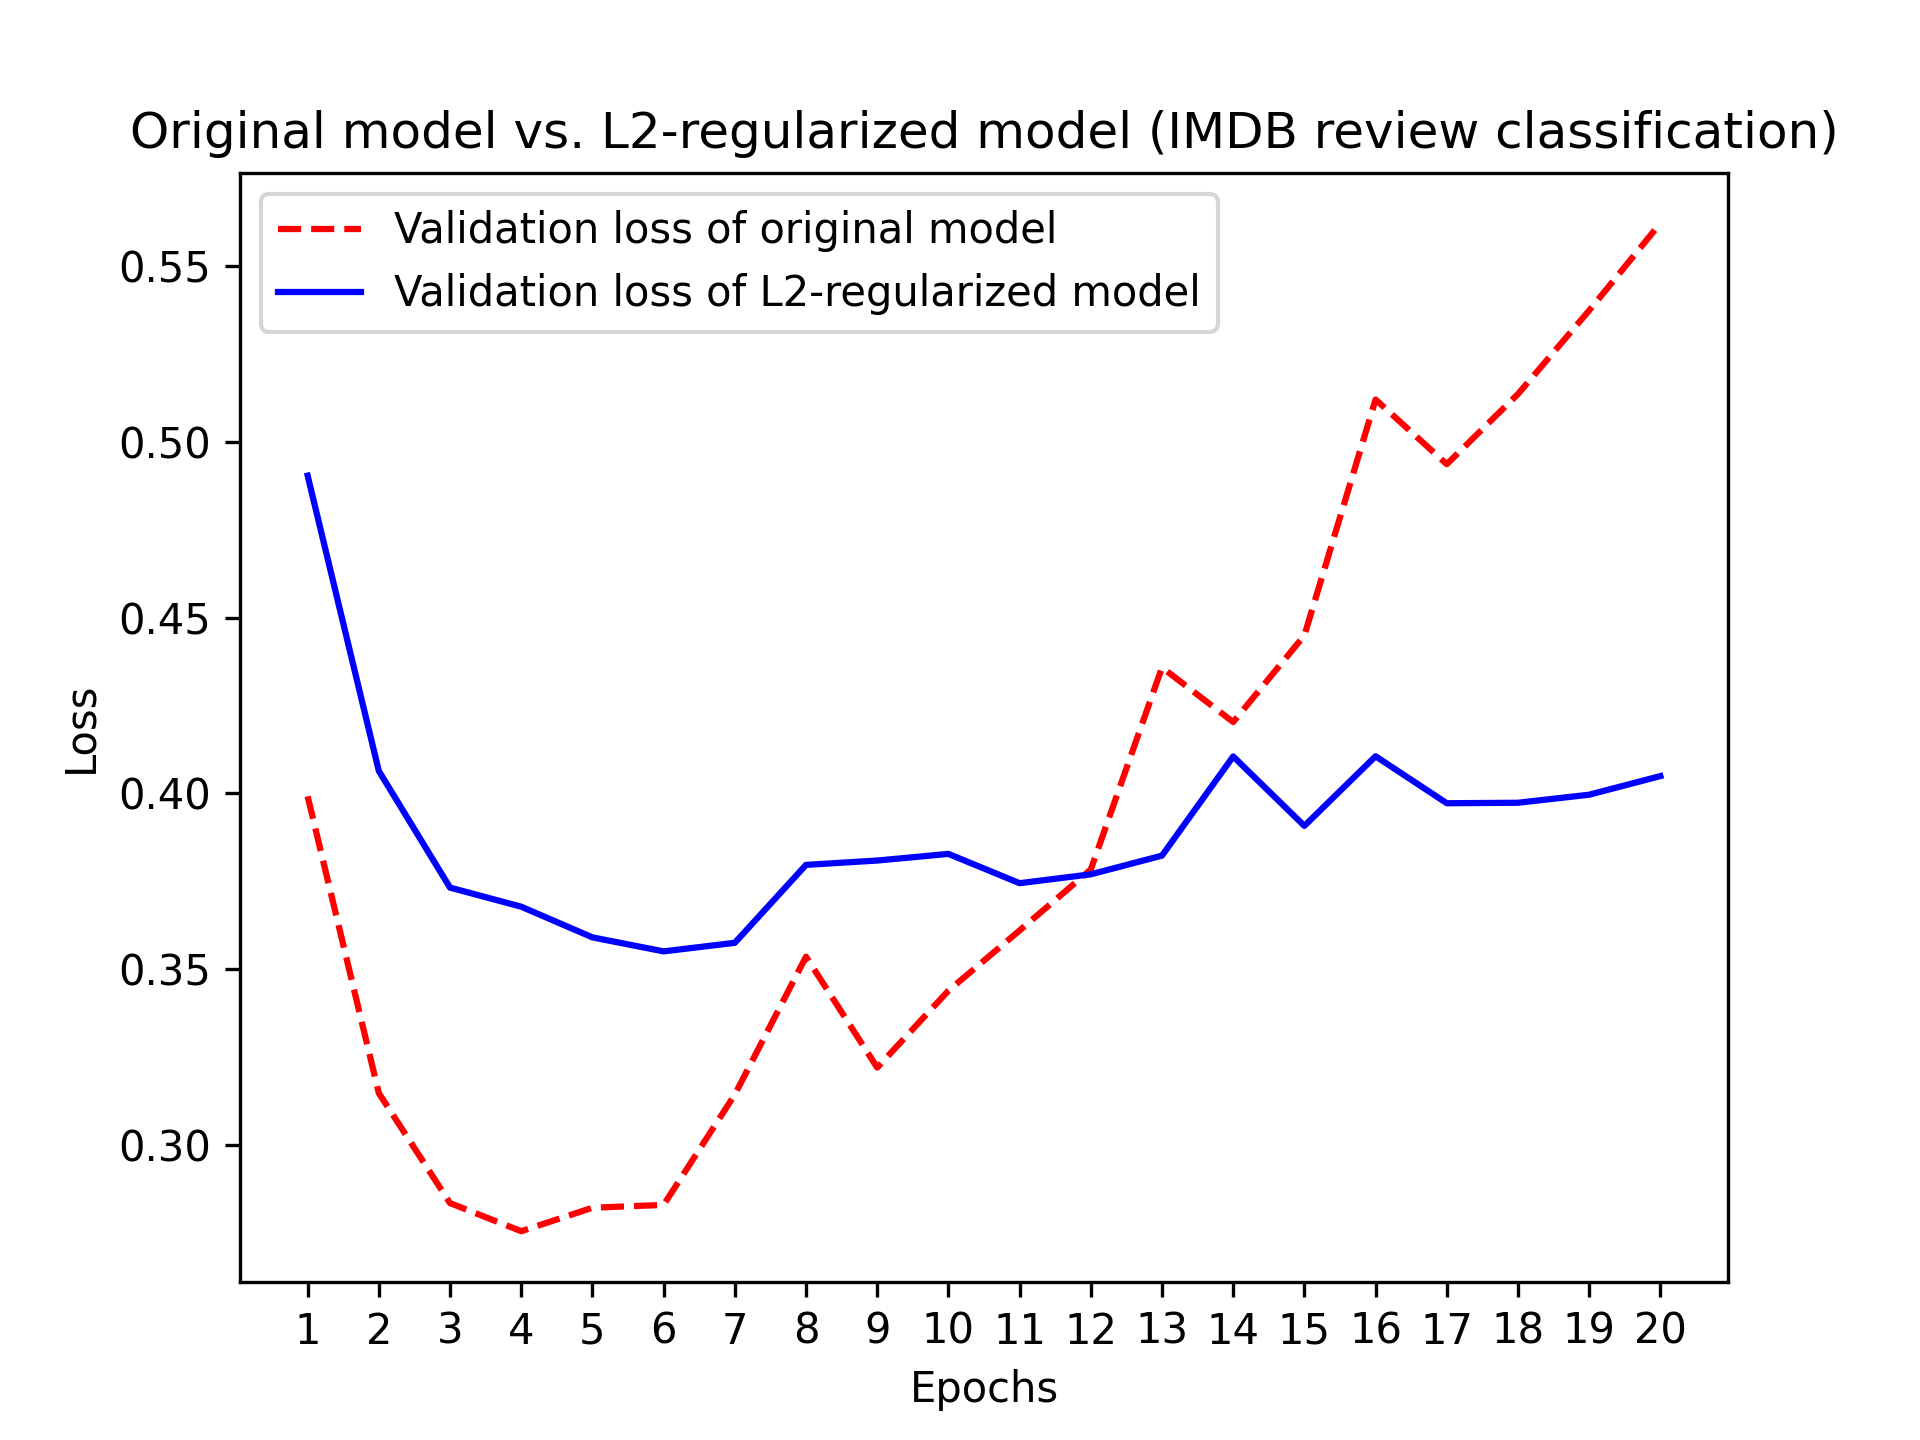
\includegraphics[width=\textwidth,height=0.7\textheight,keepaspectratio]{../../images/ch05/original_model_vs_l2_regularized_model_imdb.2b413ef1.png}
            \caption{Hiệu quả của L2 Regularization (Crosses)}
        \end{figure}
    \end{columns}
\end{frame}

\begin{frame}{Kỹ thuật Dropout (Ngắt Nơ-ron Ngẫu nhiên)}
    \begin{columns}
        \column{0.5\textwidth}
        \begin{itemize}
            \item Kỹ thuật cách mạng do \textbf{Geoffrey Hinton} phát minh. 
            \item Cơ chế: Trong từng bước tối ưu, tại một layer, đột ngột vô hiệu hóa ngẫu nhiên (ép về giá trị $0$) một tỷ lệ (rate) các nơ-ron, thường là $0.2 \sim 0.5$.
            \item Ngăn chặn hiện tượng "đồng thích nghi" (Co-adaptation): Các nơ-ron không thể ỷ lại, dựa dẫm học chung một tính năng với nơ-ron khác $\rightarrow$ Buộc phải tự hình thành những đặc trưng độc lập và mạnh mẽ.
        \end{itemize}
        
        \column{0.5\textwidth}
        \begin{figure}
            \centering
            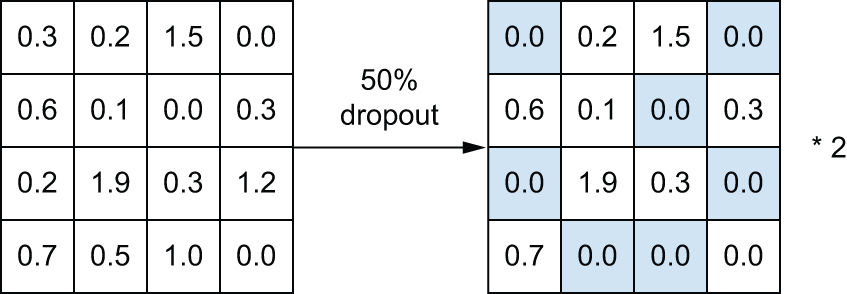
\includegraphics[width=\textwidth,height=0.7\textheight,keepaspectratio]{../../images/ch05/dropout.8e0a70b8.png}
            \caption{Quá trình Dropout tại thời điểm Training}
        \end{figure}
    \end{columns}
\end{frame}

\begin{frame}[fragile]{Cơ chế cân bằng Toán học của Dropout}
    \begin{itemize}
        \item \textbf{Khi Training:} Ngắt $50\%$ nơ-ron (rate $= 0.5$).
        \item \textbf{Khi Testing (Inference):} Tuyệt đối không Dropout! Mô hình chạy full công suất.
        \item Vấn đề: Nếu lúc học có 50 người kéo co, lúc thi có tận 100 người kéo co thì tổng lực (tổng Activation) bị tăng gấp đôi, làm vỡ hàm Loss.
        \item Giải pháp Keras: Tại lúc học, các kích hoạt còn sống sót sẽ được \textbf{Scale Up} (nhân cho $\frac{1}{1 - \text{rate}} = 2$).
    \end{itemize}
\begin{lstlisting}[language=Python]
model = keras.Sequential([
    layers.Dense(16, activation="relu"),
    layers.Dropout(0.5), # Nhet lop Dropout ngay sau lop Dense
    layers.Dense(16, activation="relu"),
    layers.Dropout(0.5),
    layers.Dense(1, activation="sigmoid")
])
\end{lstlisting}
\end{frame}


\begin{frame}{Hiệu quả của Dropout}
    \begin{columns}
        \column{0.5\textwidth}
        \begin{itemize}
            \item Trong biểu đồ này, mạng sử dụng Dropout rate $= 0.5$ (Crosses) đã kháng cự lại sự Overfit vô cùng kiên cường.
            \item Đây chính là kỹ thuật Regularization hiệu quả và được áp dụng gần như mặc định cho các mô hình Deep Learning cực sâu hiện tại.
        \end{itemize}
        
        \column{0.5\textwidth}
        \begin{figure}
            \centering
            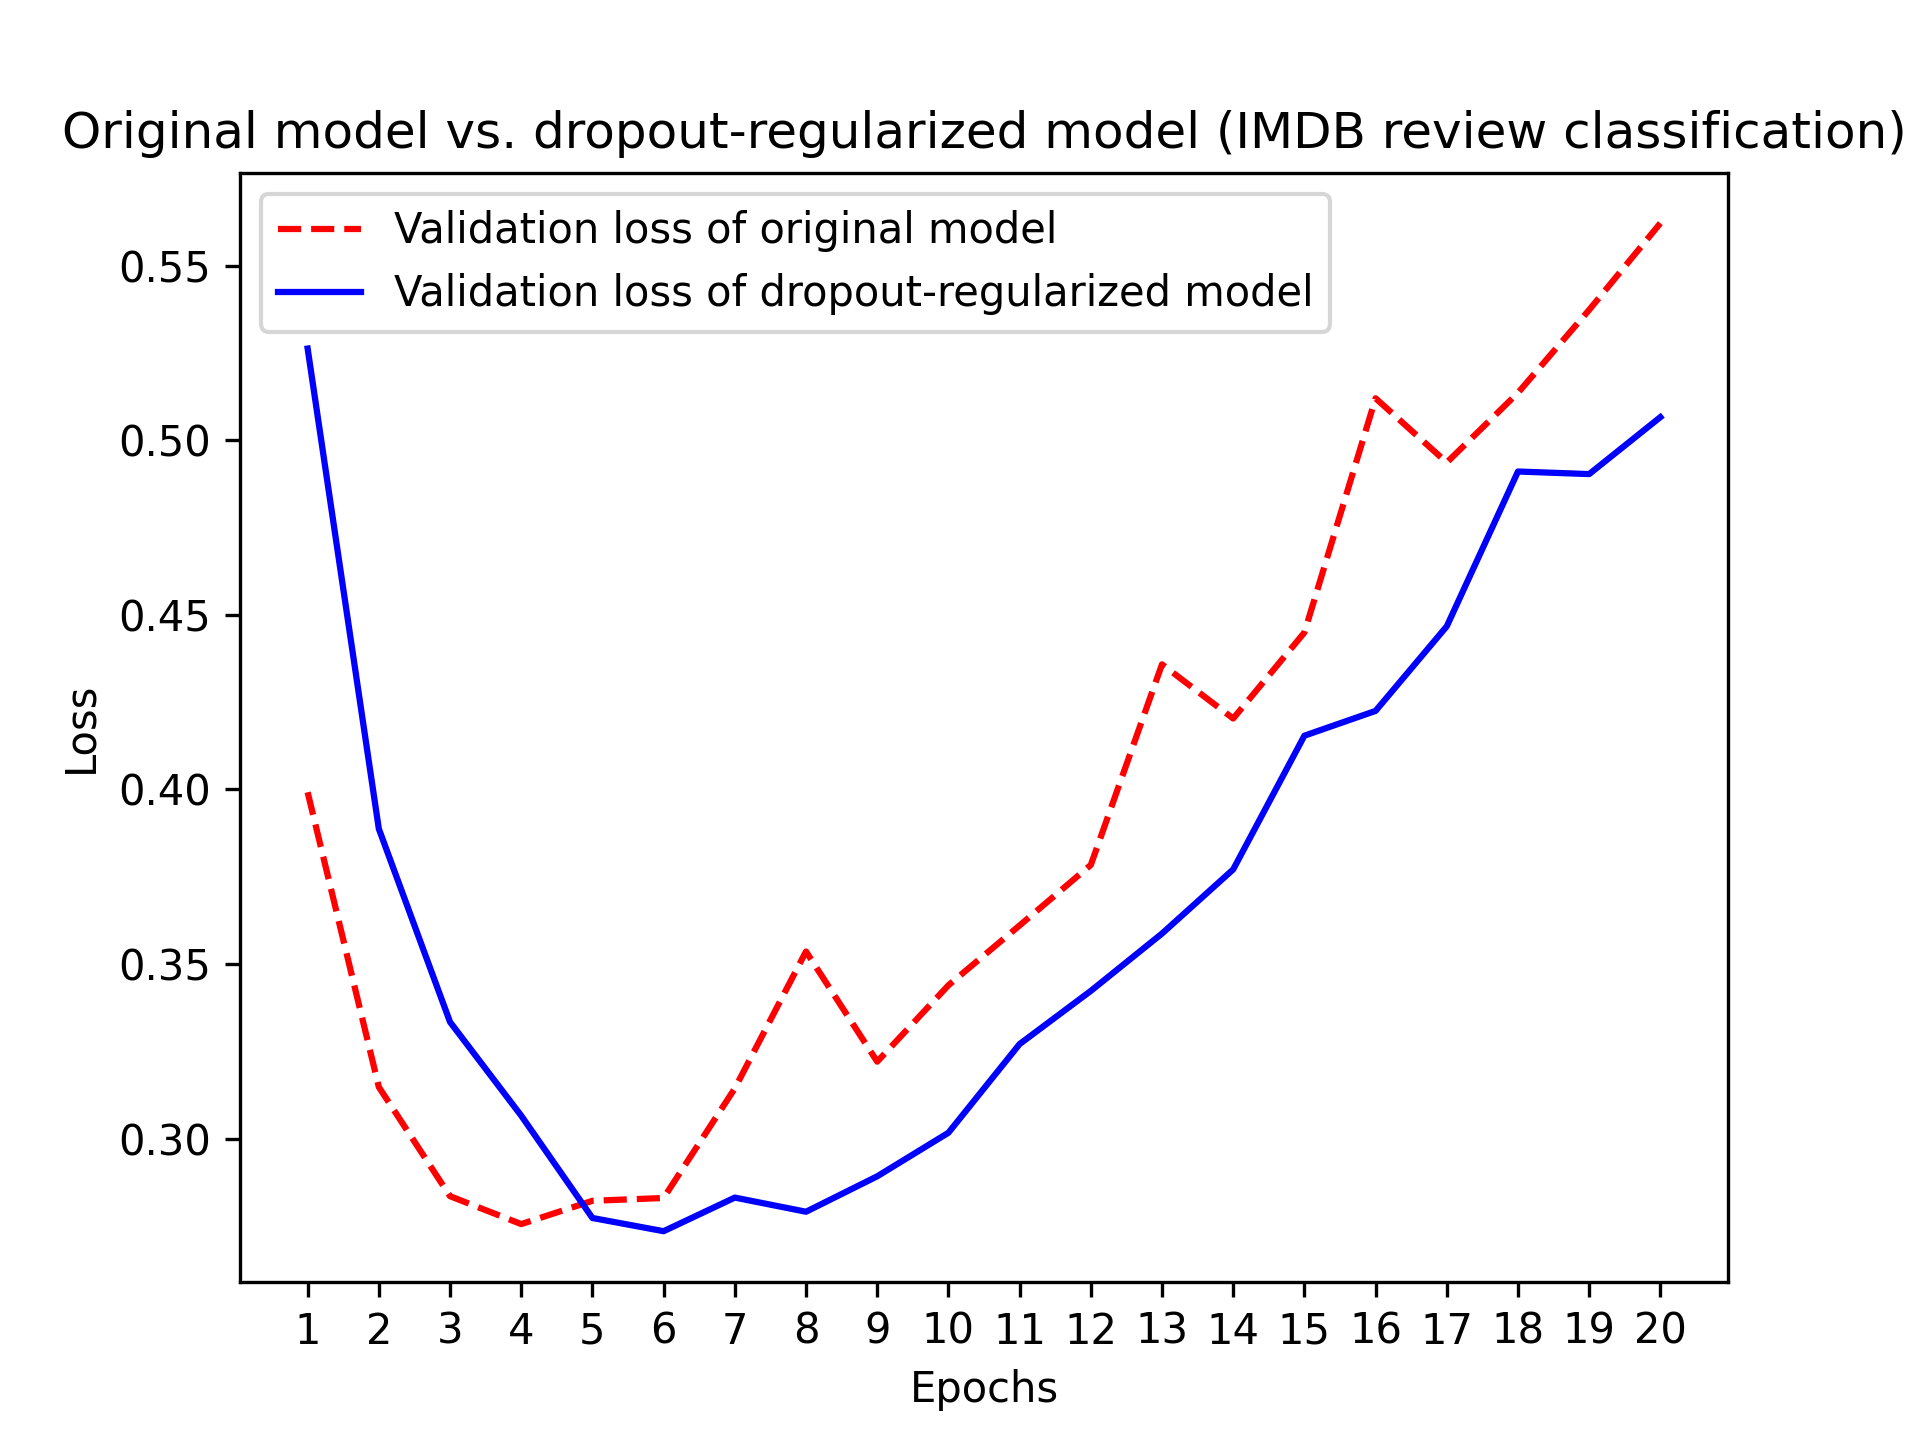
\includegraphics[width=\textwidth,height=0.7\textheight,keepaspectratio]{../../images/ch05/original_model_vs_dropout_regularized_model_imdb.58acc10b.png}
            \caption{Hiệu quả của Dropout (Crosses)}
        \end{figure}
    \end{columns}
\end{frame}

\section{6. Quản lý dữ liệu và Kỹ thuật Tính năng}

\begin{frame}{Kỹ thuật tính năng (Feature Engineering)}
    \begin{itemize}
        \item Feature Engineering là quá trình sử dụng kiến thức, quy luật chuyên gia (Domain Knowledge) để biến đổi dữ liệu đầu vào sao cho nó trở nên thân thiện nhất với thuật toán ML/DL.
        \item DL hiện đại có khả năng trích xuất tính năng ẩn một cách tự động, tuy nhiên với các tập dữ liệu nhỏ hoặc bài toán đặc thù, nếu ta thiết kế Feature Engineering tốt, mô hình sẽ tốn ít tài nguyên hơn, chạy nhanh hơn và chính xác hơn.
        \item Một bài toán kinh điển: Nhận diện thời gian trên đồng hồ kim.
    \end{itemize}
\end{frame}

\begin{frame}{Ví dụ: Bài toán đọc Đồng hồ}
    \begin{columns}
        \column{0.5\textwidth}
        \begin{itemize}
            \item \textbf{Cách 1 (Không tinh tế):} Dùng dữ liệu pixel ảnh trực tiếp, nuôi bằng mạng chập CNN. Cực kỳ lãng phí tài nguyên và dữ liệu huấn luyện khổng lồ.
            \item \textbf{Cách 2 (Trung gian):} Code Python trích xuất tọa độ $(x, y)$ của đầu kim đồng hồ. Cho thuật toán ML dễ dàng học các số tọa độ.
            \item \textbf{Cách 3 (Feature đỉnh cao):} Chuyển $(x, y)$ sang tọa độ cực: góc độ $\theta$. Lúc này, bài toán giải bằng 1 hàm làm tròn chia chẵn lẻ mà không cần AI! 
        \end{itemize}
        
        \column{0.5\textwidth}
        \begin{figure}
            \centering
            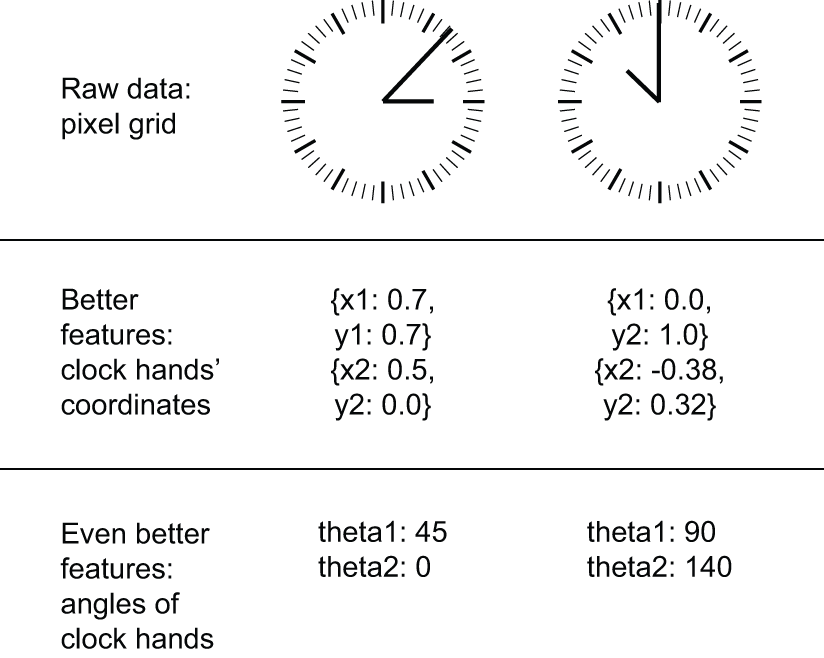
\includegraphics[width=\textwidth,height=0.7\textheight,keepaspectratio]{../../images/ch05/clock_diagram.3cbff177.png}
            \caption{Feature Engineering cho bài toán đọc thời gian}
        \end{figure}
    \end{columns}
\end{frame}

\section{7. Giả thuyết Đa tạp (The Manifold Hypothesis)}

\begin{frame}{Giả thuyết Đa tạp (The Manifold Hypothesis) là gì?}
    \begin{itemize}
        \item Một ảnh màu $256 \times 256$ có $3$ kênh màu RGB tạo ra một không gian lên tới hàng tỷ tỷ chiều (cao hơn vô hạn so với số nguyên tử trong vũ trụ). 
        \item Nếu lấy ngẫu nhiên 1 tập pixel bất kỳ, xác suất tạo ra hình dạng "hợp lý" là $0$.
        \item \textbf{Manifold Hypothesis:} Tuy nhiên, các dữ liệu có ý nghĩa thực tế của loài người (ảnh tự nhiên, khuôn mặt, chữ số MNIST, âm thanh) chỉ nằm tập trung tại một dải không gian con cấu trúc cao, uốn lượn gọn gàng, gọi là \textbf{Đa tạp (Manifold)}.
        \item Học sâu chính là quá trình vuốt phẳng dần (uncrumpling) các đa tạp rối rắm ẩn sâu này.
    \end{itemize}
\end{frame}

\begin{frame}{Nội suy Tuyến tính vs Nội suy Đa tạp}
    \begin{columns}
        \column{0.5\textwidth}
        \begin{itemize}
            \item Khi mô hình dự đoán một điểm chưa từng thấy, nó thực hiện \textbf{Nội suy (Interpolation)}.
            \item Nội suy tuyến tính (đường thẳng nối giữa 2 chữ số) thường tạo ra những giá trị văng ra ngoài không gian của chữ số $\rightarrow$ Tức là tạo ra khối hình vô nghĩa (Ảnh trái).
            \item Học sâu bám chặt vào đường cong Đa tạp, nội suy dọc theo mặt phẳng cong (Manifold Interpolation), mang lại hình chuyển tiếp siêu mượt (Ảnh phải).
        \end{itemize}
        
        \column{0.5\textwidth}
        \begin{figure}
            \centering
            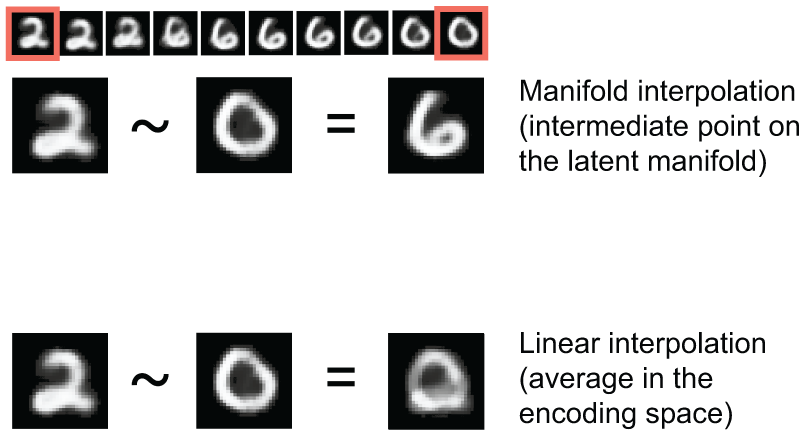
\includegraphics[width=\textwidth,height=0.7\textheight,keepaspectratio]{../../images/ch05/linear_interpolation_vs_manifold_interpolation.75960718.png}
            \caption{Linear Interpolation (sai) vs Manifold (đúng)}
        \end{figure}
    \end{columns}
\end{frame}

\begin{frame}{Mật độ Lấy mẫu (Dense Sampling)}
    \begin{columns}
        \column{0.5\textwidth}
        \begin{itemize}
            \item Vì học sâu bản chất chỉ là "khớp đường cong", nên để học được trọn vẹn Đa tạp cong uốn lượn, chúng ta cần khối lượng dữ liệu khổng lồ lấp đầy bề mặt (Dense Sampling).
            \item Không gian ẩn (Latent space) của mạng học được sẽ tự động gom cụm các chữ số theo từng đảo (cluster) giống nhau (Ảnh dưới).
            \item "Thuật toán tối tân không bù đắp được dữ liệu thưa thớt."
        \end{itemize}
        
        \column{0.5\textwidth}
        \begin{figure}
            \centering
            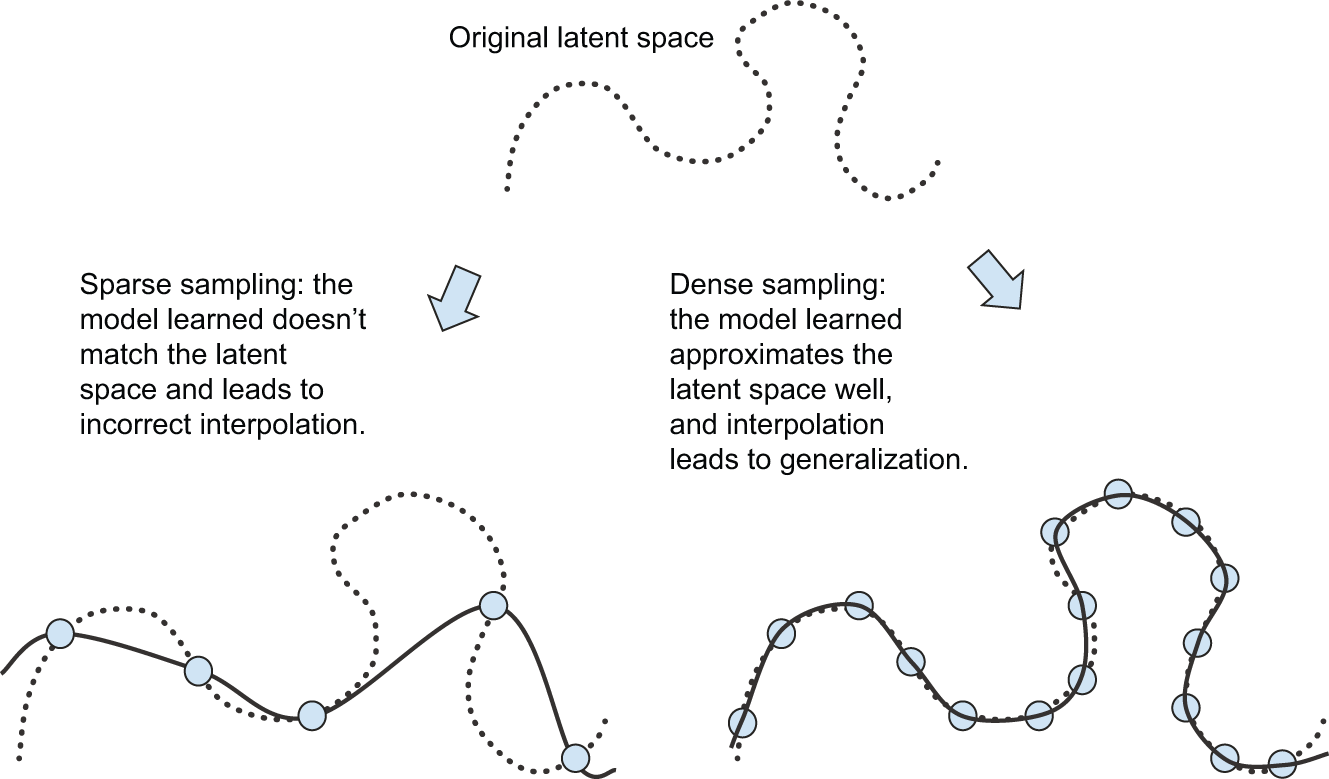
\includegraphics[width=\textwidth,height=0.45\textheight,keepaspectratio]{../../images/ch05/dense_sampling.c8a0767c.png} \\
            \vspace{0.2cm}
            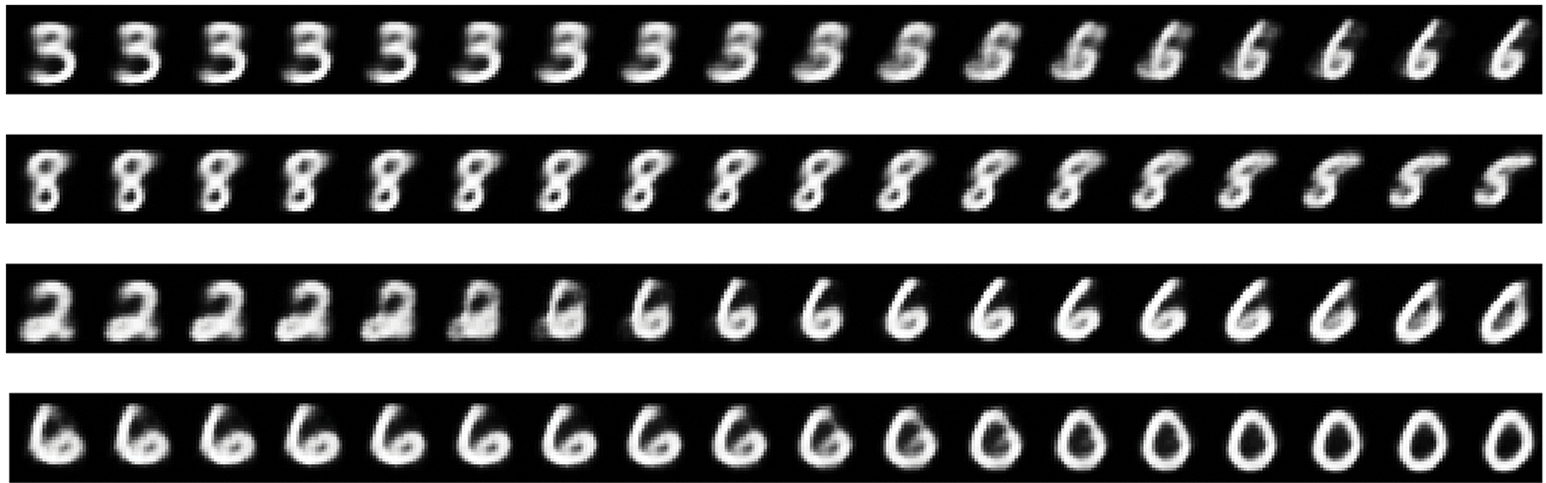
\includegraphics[width=\textwidth,height=0.45\textheight,keepaspectratio]{../../images/ch05/mnist_manifold.665acfb1.png}
            \caption{Dense Sampling \& MNIST Manifold}
        \end{figure}
    \end{columns}
\end{frame}

\section{Tổng kết}

\begin{frame}{Tổng kết Chương 5}
    \begin{itemize}
        \item Cốt lõi của Học máy là duy trì ranh giới mỏng manh giữa việc cực đại hóa \textbf{Optimization} trên tập Train mà không phá hủy \textbf{Generalization} trên tập Test.
        \item \textbf{Overfitting} luôn rình rập do dữ liệu nhiễu, do kiến trúc mạng quá dư thừa tham số.
        \item Bắt buộc áp dụng các giao thức đánh giá Hold-out hoặc K-Fold Validation đúng cách, tuyệt đối không Tuning siêu tham số trên tập Test.
        \item Khắc phục Overfit bằng vũ khí kỹ thuật:
        \begin{itemize}
            \item \textbf{Thêm Dữ liệu / Data Augmentation / Feature Engineering.}
            \item Thu nhỏ mạng (Reduce Network Capacity).
            \item Bổ sung Phạt Trọng số (\textbf{L2 Regularization}).
            \item Bổ sung Nhiễu phân tách Co-adaptation (\textbf{Dropout}).
            \item Ngừng sớm (\textbf{Early Stopping}).
        \end{itemize}
    \end{itemize}
\end{frame}

\end{document}
